%%%%%%%%%%%%%%%%%%%%%%%%%%%%%%%%%%%%%%%%%%%%%%%%%%%%%%%%%%%%%%%%%%%%%%%%%%
%Author:																 %
%-------																 %
%Yannis Baehni at University of Zurich									 %
%baehni.yannis@uzh.ch													 %
%																		 %
%Version log:															 %
%------------															 %
%06/02/16 . Basic structure												 %
%04/08/16 . Layout changes including section, contents, abstract.		 %
%%%%%%%%%%%%%%%%%%%%%%%%%%%%%%%%%%%%%%%%%%%%%%%%%%%%%%%%%%%%%%%%%%%%%%%%%%

%Page Setup
\documentclass[
	12pt, 
	oneside, 
	a4paper,
	reqno,
	final
]{amsbook}

\usepackage[
	left = 3cm, 
	right = 3cm, 
	top = 3cm, 
	bottom = 3cm
]{geometry}

%Headers and footers
\newcommand\hmmax{0}
\newcommand\bmmax{0}

%Title
\usepackage[foot]{amsaddr}
\usepackage{newtxtext}
\usepackage[subscriptcorrection,nofontinfo,mtpcal,mtphrb]{mtpro2}
\usepackage{mathtools}
\usepackage{bm}
\usepackage{xspace}
\usepackage[all]{xy}
\usepackage{tikz-cd}
\usepackage{xcolor}
\usepackage{setspace}

\makeindex

\makeatletter
\def\@textbottom{\vskip \z@ \@plus 1pt}
\let\@texttop\relax
\usepackage{etoolbox}
\patchcmd{\abstract}{\scshape\abstractname}{\textbf{\abstractname}}{}{}
\usepackage{chngcntr}
\counterwithout{figure}{chapter}
%Section, subsection and subsubsection font
%------------------------------------------
	\renewcommand{\@secnumfont}{\bfseries}
	\renewcommand\section{\@startsection{section}{1}%
  	\z@{.7\linespacing\@plus\linespacing}{.5\linespacing}%
  	{\normalfont\bfseries\boldmath\centering}}
	\renewcommand\subsection{\@startsection{subsection}{2}%
    	\z@{.5\linespacing\@plus.7\linespacing}{-.5em}%
    	{\normalfont\bfseries\boldmath}}%
	\renewcommand\subsubsection{\@startsection{subsubsection}{3}%
    	\z@{.5\linespacing\@plus.7\linespacing}{-.5em}%
    	{\normalfont\bfseries\boldmath}}%

		\renewenvironment{proof}{\noindent\textit{Proof}.}{\qed}

%ToC
%---
\makeatletter
\setcounter{tocdepth}{3}
% Add bold to \chapter titles in ToC and remove . after numbers
\renewcommand{\tocchapter}[3]{%
  	\indentlabel{\@ifnotempty{#2}{\bfseries\ignorespaces#1 #2: }}\bfseries#3}
\renewcommand{\tocappendix}[3]{%
  	\indentlabel{\@ifnotempty{#2}{\bfseries\ignorespaces#1 #2: }}\bfseries#3}
% Remove . after numbers in \section and \subsection
\renewcommand{\tocsection}[3]{%
  	\indentlabel{\@ifnotempty{#2}{\ignorespaces#1 #2\quad}}#3}
\renewcommand{\tocsubsection}[3]{%
  	\indentlabel{\@ifnotempty{#2}{\ignorespaces#1 #2\quad}}#3}
\let\tocsubsubsection\tocsubsection% Update for \subsubsection
%...
\newcommand\@dotsep{4.5}
\def\@tocline#1#2#3#4#5#6#7{\relax
  \ifnum #1>\c@tocdepth % then omit
  \else
    \par \addpenalty\@secpenalty\addvspace{#2}%
    \begingroup \hyphenpenalty\@M
    \@ifempty{#4}{%
      \@tempdima\csname r@tocindent\number#1\endcsname\relax
    }{%
      \@tempdima#4\relax
    }%
    \parindent\z@ \leftskip#3\relax \advance\leftskip\@tempdima\relax
    \rightskip\@pnumwidth plus1em \parfillskip-\@pnumwidth
    #5\leavevmode\hskip-\@tempdima{#6}\nobreak
    \leaders\hbox{$\m@th\mkern \@dotsep mu\hbox{.}\mkern \@dotsep mu$}\hfill
    \nobreak
    \hbox to\@pnumwidth{\@tocpagenum{\ifnum#1=0\bfseries\fi#7}}\par% <-- \bfseries for \chapter page
    \nobreak
    \endgroup
  \fi}
\AtBeginDocument{%
\expandafter\renewcommand\csname r@tocindent0\endcsname{0pt}
}
\def\l@subsection{\@tocline{2}{0pt}{2.5pc}{5pc}{}}
\def\l@subsubsection{\@tocline{2}{0pt}{4.5pc}{5pc}{}}
\makeatother

\advance\footskip0.4cm
\textheight=54pc    %a4paper
\textheight=50.5pc %letterpaper
\advance\textheight-0.4cm
\calclayout

%Font settings
%\usepackage{anyfontsize}
%Footnote settings
\usepackage{footmisc}
%	\renewcommand*{\thefootnote}{\fnsymbol{footnote}}
\usepackage{commath}
%Further math environments
%Further math fonts (loads amsfonts implicitely)
%Redefinition of \text
%\usepackage{amstext}
\usepackage{upref}
%Graphics
%\usepackage{graphicx}
%\usepackage{caption}
%\usepackage{subcaption}
%Frames
\usepackage{mdframed}
\allowdisplaybreaks
%\usepackage{interval}
\newcommand{\toup}{%
  \mathrel{\nonscript\mkern-1.2mu\mkern1.2mu{\uparrow}}%
}
\newcommand{\todown}{%
  \mathrel{\nonscript\mkern-1.2mu\mkern1.2mu{\downarrow}}%
}
\AtBeginDocument{\renewcommand*\d{\mathop{}\!\mathrm{d}}}
\renewcommand{\Re}{\operatorname{Re}}
\renewcommand{\Im}{\operatorname{Im}}
\DeclareMathOperator\Log{Log}
\DeclareMathOperator\Arg{Arg}
\DeclareMathOperator\id{id}
\DeclareMathOperator\sech{sech}
\DeclareMathOperator\Aut{Aut}
\DeclareMathOperator\h{h}
\DeclareMathOperator\sgn{sgn}
\DeclareMathOperator\arctanh{arctanh}
\DeclareMathOperator\supp{supp}
\DeclareMathOperator\ob{ob}
\DeclareMathOperator\mor{mor}
\DeclareMathOperator\M{M}
\DeclareMathOperator\dom{dom}
\DeclareMathOperator\cod{cod}
\DeclareMathOperator\im{im}
\DeclareMathOperator\Ab{Ab}
\DeclareMathOperator\coker{coker}
\DeclareMathOperator\Cone{Cone}
\DeclareMathOperator\diam{diam}
\DeclareMathOperator\Tor{Tor}
\DeclareMathOperator\Ch{Ch}
\DeclareMathOperator\Hom{Hom}
\DeclareMathOperator\Ho{Ho}
\DeclareMathOperator\End{End}

\makeatletter
\newcommand{\colim@}[2]{%
  \vtop{\m@th\ialign{##\cr
    \hfil$#1\operator@font colim$\hfil\cr
    \noalign{\nointerlineskip\kern1.5\ex@}#2\cr
    \noalign{\nointerlineskip\kern-\ex@}\cr}}%
}
\newcommand{\colim}{%
  \mathop{\mathpalette\colim@{\rightarrowfill@\textstyle}}\nmlimits@
}
\makeatother
%\usepackage{hhline}
%\usepackage{booktabs} 
%\usepackage{array}
%\usepackage{xfrac} 
%\everymath{\displaystyle}
%Enumerate
\usepackage{tikz}
%\usepackgae{graphicx}
\usepackage{subcaption}
\makeatletter
\def\@captionheadfont{}
\makeatother
\renewcommand{\thesubfigure}{\alph{subfigure}}
\usepackage{enumitem} 
%\renewcommand{\labelitemi}{$\bullet$}
%\renewcommand{\labelitemii}{$\ast$}
%\renewcommand{\labelitemiii}{$\cdot$}
%\renewcommand{\labelitemiv}{$\circ$}
%Colors
%\usepackage{color}
%\usepackage[cmtip, all]{xy}
%Main style theorem environment
\newtheoremstyle{main} 		             	 		%Stylename
  	{}	                                     		%Space above
  	{}	                                    		%Space below
  	{\itshape}			                     		%Body font
  	{}        	                             		%Indent
  	{\bfseries\boldmath}   	                         		%Head font
  	{.}            	                        		%Head punctuation
  	{ }           	                         		%Head space 
  	{\thmname{#1}\thmnumber{ #2}\thmnote{ (#3)}}	%Head specification
\theoremstyle{main}
\newtheorem{theorem}{Theorem}[chapter]
\newtheorem{definition}[theorem]{Definition}
\newtheorem{proposition}[theorem]{Proposition}
\newtheorem{corollary}[theorem]{Corollary}
\newtheorem{lemma}[theorem]{Lemma}
\newtheorem{axiom}{Axiom}
\newtheoremstyle{nonit} 		             	 		%Stylename
  	{}	                                     		%Space above
  	{}	                                    		%Space below
  	{}			                     		%Body font
  	{}        	                             		%Indent
  	{\bfseries\boldmath}   	                   		%Head font
  	{.}            	                        		%Head punctuation
  	{ }           	                         		%Head space 
  	{\thmname{#1}\thmnumber{ #2}\thmnote{ (#3)}}	%Head specification
\theoremstyle{nonit}
\newtheorem{remark}[theorem]{Remark}
\newtheorem{examples}[theorem]{Examples}
\newtheorem{example}[theorem]{Example}
\newtheorem{problem}{Problem}[chapter]
\newtheoremstyle{ex} 		             	 		%Stylename
  	{}	                                     		%Space above
  	{}	                                    		%Space below
  	{\small}			                     		%Body font
  	{}        	                             		%Indent
  	{\bfseries\boldmath}   	                         		%Head font
  	{.}            	                        		%Head punctuation
  	{ }           	                         		%Head space 
  	{\thmname{#1}\thmnumber{ #2}\thmnote{ (#3)}}	%Head specification
\theoremstyle{ex}
\newtheorem{exercise}[theorem]{Exercise}
%German non-ASCII-Characters
%Graphics-Tool
%\usepackage{tikz}
%\usepackage{tikzscale}
%\usepackage{bbm}
%\usepackage{bera}
%Listing-Setup
%Bibliographie
\usepackage[backend=bibtex, style=alphabetic]{biblatex}
%\usepackage[babel, german = swiss]{csquotes}
\bibliography{bibliography}
%PDF-Linking
%\usepackage[hyphens]{url}
\usepackage[bookmarksopen=true,bookmarksnumbered=true]{hyperref}
%\PassOptionsToPackage{hyphens}{url}\usepackage{hyperref}
\urlstyle{rm}
\hypersetup{
  colorlinks   = true, %Colours links instead of ugly boxes
  urlcolor     = blue, %Colour for external hyperlinks
  linkcolor    = blue, %Colour of internal links
  citecolor    = blue %Colour of citations
}
\newcommand{\bld}[1]{\boldmath\textit{\textbf{#1}}\unboldmath}
\newcommand{\eqclass}[1]{\sbr[0]{#1}}
\newcommand{\cat}[1]{\mathsf{#1}}
\newcommand{\Sbb}{\mathbb{S}}
\newcommand{\Zbb}{\mathbb{Z}}
\newcommand{\Nbb}{\mathbb{N}}
\newcommand{\Rbb}{\mathbb{R}}
\newcommand{\Hbb}{\mathbb{H}}
\newcommand{\Cbb}{\mathbb{C}}
\newcommand{\Tcal}{\mathcal{T}}
\newcommand{\SLrm}{\mathrm{SL}}
\newcommand{\PSLrm}{\mathrm{PSL}}
\newcommand{\SLrmstar}{\mathrm{S^*L}}
\newcommand{\PSLrmstar}{\mathrm{PS^*L}}
\newcommand{\GLrm}{\mathrm{GL}}
\newcommand{\Mrm}{\mathrm{M}}
\newcommand{\Isom}{\mathrm{Isom}}
\newcommand{\Mob}{\mathrm{M\ddot{o}b}}
\newcommand{\Ebb}{\mathbb{E}}
\newcommand{\Cscr}{\mathscr{C}}
\newcommand{\pwrm}{\mathrm{pw}}
\newcommand{\clos}[1]{\overline{#1}}
\newcommand{\Hcal}{\mathcal{H}}
\newcommand{\Hbcal}{\bm{\mathcal{H}}}
\newcommand{\Ucal}{\mathcal{U}}
\newcommand{\Ubcal}{\bm{\mathcal{U}}}
\renewcommand{\det}{\mathrm{det}}
\newcommand{\ab}{\mathrm{ab}}
\newcommand{\op}{\mathrm{op}}

\usepackage{trimclip}
\newcommand{\crop}[1]{\clipbox*{0pt -.5ex {\width} {.7\height}}{#1}}
\newcommand{\jota}{\crop{\raisebox{-2pt}{\scalebox{1}[1.5]{\rotatebox[origin=c]{-32}{\reflectbox{$\iota$}}}}}}



\begin{document}

%Roman page numbering
\frontmatter

\renewcommand*{\thefootnote}{\fnsymbol{footnote}}

%Half-Title Page
\thispagestyle{empty}

\begin{center}
    \rule{\linewidth}{1mm}\\
	\fontsize{85}{85}{\textsc{Classical Mechanics}}\\
	\rule{\linewidth}{1mm} \\[.5cm]
	\fontsize{25}{25}{\textsc{Yannis B\"ahni\footnote{ETH Z\"urich, R\"amistrasse 101, 8092 Z\"urich. \emph{E-mail address}: \href{mailto:baehniy@student.ethz.ch}{\nolinkurl{baehniy@student.ethz.ch}}}}}\\
	\vspace{5cm}
	Semester Paper under the Supervision of Prof. Dr. Ana Cannas Da Silva at ETH Z\"urich
\end{center}
\clearpage

\chapter*{Preface}
\noindent Winterthur, \hfill Yannis B\"ahni\\
September 8, 2018
\tableofcontents

\mainmatter

\renewcommand*{\thefootnote}{\arabic{footnote}}

\chapter{Lagrangian Mechanics}

\section*{Introduction}
Classical mechanics deals with differential equations originating from extremals of \emph{functionals}, i.e. functions defined on an infinite-dimensional function space. The study of such extremality properties of functionals is known as the \emph{calculus of variations}. To illustrate this fundamental principle, let us consider the \emph{variational formulation} of second order elliptic operators in divergence form based on \cite[167--168]{struwe:fa:2014}.\\ 
Let $n \in \mathbb{N}$, $n \geq 1$, and $\Omega \subseteq \subseteq \mathbb{R}^n$ such that $\wbar{\Omega}$ is a manifold with boundary. Moreover, let $H^1_0(\Omega)$ denote the Sobolev space $W^{1,2}_0(\Omega)$ with inner product
\begin{equation*}
	\langle u,v \rangle_{H^1_0(\Omega)} = \int_\Omega uv + \int_\Omega \nabla u \nabla v.
\end{equation*}
Suppose $a^{ij} \in C^\infty(\wbar{\Omega})$ symmetric, $f \in C^\infty(\wbar{\Omega})$ and consider the second order homogenous Dirichlet problem
\begin{equation}
	\label{eq:homogeneous_Dirichlet_problem}
	\ccases{
			\displaystyle -\frac{\partial}{\partial x^j}\del[3]{a^{ij}\frac{\partial u}{\partial x^i}} = f & \text{in } \Omega,\\
			u = 0 & \text{on } \partial \Omega,
		}
\end{equation}
Suppose $u \in C^\infty(\wbar{\Omega})$ solves (\ref{eq:homogeneous_Dirichlet_problem}). Then integration by parts (see \cite[436]{lee:smooth_manifolds:2013}) yields 
\begin{equation*}
	\int_\Omega f v = -\int_\Omega \frac{\partial}{\partial x^j}\del[3]{a^{ij}\frac{\partial u}{\partial x^i}}v = -\int_\Omega \mathrm{div}(X)v = \int_\Omega \langle X, \nabla v\rangle = \int_\Omega a^{ij} \frac{\partial u}{\partial x^i}\frac{\partial v}{\partial x^j}
\end{equation*}
\noindent for any $v \in C^\infty_c(\Omega)$, where $X := \del[1]{a^{ij}\frac{\partial u}{\partial x^i}}_j$. Thus we say that $u \in H^1_0(\Omega)$ is a \emph{weak solution} of (\ref{eq:homogeneous_Dirichlet_problem}) iff
\begin{equation*}
	\forall v \in C^\infty_c(\Omega): \> \int_\Omega a^{ij} \frac{\partial u}{\partial x^i}\frac{\partial v}{\partial x^j} = \int_\Omega fv.
\end{equation*}
If $(a^{ij})_{ij}$ is \emph{uniformly elliptic}, i.e. there exists $\lambda > 0$ such that
\begin{equation*}
	\forall x \in \Omega\forall \xi \in \mathbb{R}^n : \> a^{ij}(x)\xi_i\xi_j \geq \lambda \abs{\xi}^2,	
\end{equation*}
\noindent then (\ref{eq:homogeneous_Dirichlet_problem}) admits a unique weak solution $u \in H^1_0(\Omega)$ (in fact $u \in C^\infty(\Omega)$ using \emph{regularity theory}, for more details see \cite[175]{struwe:fa:2014}). Indeed, observe that 
\begin{equation*}
	\langle \cdot,\cdot \rangle_a : H^1_0(\Omega) \times H^1_0(\Omega) \to \mathbb{R}
\end{equation*}
\noindent defined by
\begin{equation}
	\label{eq:Sobolev_inner_product}
	\langle u, v \rangle_a := \int_\Omega a^{ij} \frac{\partial u}{\partial x^i}\frac{\partial v}{\partial x^j}
\end{equation}
\noindent is an inner product on $H^1_0(\Omega)$ with induced norm equivalent to the standard one on $H^1_0(\Omega)$ due to Poincar\'e's inequality \cite[107]{struwe:fa:2014}. Applying the Riesz Representation theorem \cite[49--50]{struwe:fa:2014} yields the result. Moreover, this solution can be characterized by a \emph{variational principle}, i.e. if we define the \emph{energy functional} $E : H^1_0(\Omega) \to \mathbb{R}$
\begin{equation*}
	E(v) := \frac{1}{2} \norm{v}^2_a - \int_\Omega fv,
\end{equation*}
\noindent for any $v \in H^1_0(\Omega)$, where $\norm{\cdot}_a$ denotes the norm induced by the inner product (\ref{eq:Sobolev_inner_product}), then $u \in H^1_0(\Omega)$ solves (\ref{eq:homogeneous_Dirichlet_problem}) if and only if
\begin{equation}
	\label{eq:variational_formulation}
	E(u) = \inf_{v \in H^1_0(\Omega)}E(v).
\end{equation}
Indeed, suppose $u \in H^1_0(\Omega)$ is a solution of (\ref{eq:homogeneous_Dirichlet_problem}). Let $v \in H^1_0(\Omega)$. Then $u = v + w$ for $w := u - v \in H^1_0(\Omega)$ and we compute
\begin{equation*}
	E(v) = E(u + w) = \frac{1}{2}\norm{u}^2_a + \langle u,w \rangle_a + \frac{1}{2}\norm{w}^2_a - \int_\Omega f(u + w) = E(u) + \frac{1}{2}\norm{w}^2_a \geq E(u)
\end{equation*}
\noindent with equality if and only if $u = v$ a.e. Conversly, suppose the infimum is attained by some $u \in H^1_0(\Omega)$. Thus by elementary calculus
\begin{equation}
	\label{eq:derivative}
	0 = \frac{d}{dt}\bigg\vert_{t = 0} E(u + tv) = \langle u, v \rangle_a - \int_\Omega f v
\end{equation}
\noindent for all $v \in H^1_0(\Omega)$.\\
Suppose now that $u \in C^\infty(\wbar{\Omega})$ with $u\vert_{\partial \Omega} = 0$ solves the variational formulation (\ref{eq:variational_formulation}). Then again integration by parts yields
\begin{equation*}
	\langle u, v \rangle_a - \int_\Omega f v = -\int_\Omega \mathrm{div}(X) v - \int_\Omega fv = \int_\Omega \del[3]{-\frac{\partial}{\partial x^j}\del[3]{a^{ij}\frac{\partial u}{\partial x^i}} - f} v
\end{equation*}
\noindent for all $v \in C^\infty_c(\Omega)$ and where $X := \del[1]{a^{ij}\frac{\partial u}{\partial x^i}}_j$. Hence (\ref{eq:derivative}) implies 
\begin{equation*}
	\forall v \in C^\infty_c(\Omega): \> \int_\Omega \del[3]{-\frac{\partial}{\partial x^j}\del[3]{a^{ij}\frac{\partial u}{\partial x^i}} - f} v = 0.
\end{equation*}

We might expect that this implies 
\begin{equation*}
	-\frac{\partial}{\partial x^j}\del[3]{a^{ij}\frac{\partial u}{\partial x^i}} = f.
\end{equation*}

That this is indeed the case, is guaranteed by a foundational result in the \emph{calculus of variations} (therefore the name).

\begin{proposition}[Fundamental Lemma of Calculus of Variations]
	\label{prop:fundamental_lemma}
	Let $\Omega \subseteq \mathbb{R}^n$ open and $f \in L^1_{\mathrm{loc}}(\Omega)$. If
	\begin{equation*}
		\forall \varphi \in C^\infty_c(\Omega): \> \int_\Omega f\varphi = 0,
	\end{equation*}
	\noindent then $f = 0$ a.e.
\end{proposition}

\begin{proof}
	See \cite[40]{struwe:fa:2014}.
\end{proof}

Thus we recovered a second order partial differential equation from the variational formulation. In fact, this is exactly the boundary value problem (\ref{eq:homogeneous_Dirichlet_problem}) from the beginning of our exposition. This technique, and in particular the fundamental lemma of calculus of variations \ref{prop:fundamental_lemma} will play an important role in our treatment of classical mechanics. However, since we are concerned with smooth manifolds, we use a version of the fundamental lemma of calculus of variations \ref{prop:fundamental_lemma}, which is fairly easy to prove and hence really deserves the terminology lemma.

\begin{lemma}[Fundamental Lemma of Calculus of Variations, Smooth Version]
	\label{lem:fundamental_lemma}
	Let $\Omega \subseteq \mathbb{R}^n$ open and $f \in C^\infty(\Omega)$. If
	\begin{equation*}
		\forall \varphi \in C^\infty_c(\Omega): \> \int_\Omega f\varphi = 0,
	\end{equation*}
	\noindent then $f = 0$.
\end{lemma}

\begin{proof}
	Towards a contradiction, assume that $f \neq 0$ on $\Omega$. Thus there exists $x_0 \in \Omega$, such that $f(x_0) \neq 0$. Without loss of generality, we may assume that $f(x_0) > 0$, since otherwise, consider $-f$ instead of $f$.	The smoothness of $f$ implies the continuity of $f$ on $\Omega$. Thus there exists $\delta > 0$, such that $f(x) \in B_{f(x_0)/2}\del[1]{f(x_0)}$ holds for all $x \in B_\delta(x_0)$ or equivalently, $f(x) > f(x_0)/2 > 0$ for all $x \in B_\delta(x_0)$. By lemma $2.22$ \cite[42]{lee:smooth_manifolds:2013}, there exists a smooth bump function $\varphi$ supported in $B_\delta(x_0)$ and $\varphi = 1$ on $\wbar{B}_{\delta/2}(x_0)$. In particular, $\varphi \in C^\infty_c(\Omega)$. Therefore we have
	\begin{equation*}
		0 = \int_\Omega f \varphi = \int_{B_\delta(x_0)} f \varphi \geq \int_{B_{\delta/2}(x_0)} f \varphi > \frac{1}{2}f(x_0) \abs[0]{B_{\delta/2}(x_0)} > 0,
	\end{equation*}
	\noindent which is a contradiction.
\end{proof}

\begin{exercise}\footnote{This is exercise $1.2. (b)$ from exercise sheet $1$ of the course \emph{Functional Analysis II} taught by \emph{Prof. Dr. A. Carlotto} at ETHZ in the spring of 2018, which can be found \href{https://metaphor.ethz.ch/x/2018/fs/401-3462-00L/ex/Problems01-FAII.pdf}{here}.}
	Let $\Omega \subseteq \subseteq \mathbb{R}^n$, $2 \leq p < \infty$ and define $\mathcal{B} := \cbr[0]{v \in C^\infty(\wbar{\Omega}) : v\vert_{\partial\Omega} = 0}$. Moreover, define $E_p : \mathcal{B} \to \mathbb{R}$ by $E_p(v) := \int_\Omega \abs[0]{\nabla v}^p$. Derive the partial differential equation satisfied by minimizers $u \in \mathcal{B}$ of the variational problem $E(u) = \inf_{v \in \mathcal{B}}E(v)$.	
\end{exercise}

\section*{Lagrangian Systems and the Principle of Least Action}
Mechanical systems, for example a pendulum, are modelled using the language of differential geometry. Thus it is necessary to introduce the relevant physical counterparts. 

\begin{definition}[Configuration Space]
	A \bld{configuration space}\index{Configuration space} is defined to be a finite-dimensional smooth manifold.
\end{definition}

\begin{definition}[Motion]
	A \bld{motion in a configuration space $M$}\index{Motion} is defined to be a path $\gamma \in C^\infty(J, M)$, where $J \subseteq \mathbb{R}$ is an interval.
\end{definition}

\begin{definition}[State]
	A \bld{state of the configuration space}\index{State} is defined to be an element of the tangent bundle of the configuration space, called the \bld{state space}\index{Space!state}.
\end{definition}

One should think of a state $(x,v)$ of a configuration space as follows: $x$ gives the position of the mechanical system and $v$ its velocity. The fundamental principle governing motions of mechanical systems is the following.

\begin{axiom}[Newton-Laplace Determinacy Principle]
	\label{ax:NL_determinacy_principle}
	A motion in a configuration space is completely determined by a state at some instant of time.
\end{axiom}

The Newton-Laplace determinacy principle \ref{ax:NL_determinacy_principle} motivates our main definition of this chapter.

\begin{definition}[Lagrangian System]
	A \bld{Lagrangian system}\index{Lagrangian!system} is defined to be a tuple $(M,L)$ consisting of a smooth manifold $M$ and a function $L \in C^\infty(TM \times \mathbb{R})$, called a \bld{Lagrangian function}\index{Lagrangian!function}.
\end{definition}

\begin{example}
	\label{ex:Lagrangian}
	For a smooth manifold $M$ let $T \in C^\infty(TM \times \mathbb{R})$ and $V \in C^\infty(M \times \mathbb{R})$. Define $L \in C^\infty(TM \times \mathbb{R})$ by $L := T - V$. In this situation, $T$ is called the \bld{kinetic energy}\index{Energy!kinetic} and $V$ is called the \bld{potential energy}\index{Energy!potential}.
\end{example}

\begin{definition}[Path Space]
	\label{def:path_space}
	Let $M$ be a smooth manifold, $x_0,x_1 \in M$ and $t_0, t_1 \in \mathbb{R}$ with $t_0 \leq t_1$. Define the \bld{path space of $M$ connecting $(x_0,t_0)$ and $(x_1,t_1)$}\index{Space!path} to be the set
	\begin{equation}
		\label{eq:path_space}
		\mathcal{P}(M)^{x_0,t_0}_{x_1,t_1} := \cbr[0]{\gamma \in C^\infty(\intcc[0]{t_0,t_1},M) : \gamma(t_0) = x_0 \text{ and } \gamma(t_1) = x_1}.
	\end{equation}
\end{definition}

\begin{remark}
	For the sake of simplicity, we will just use the terminology \emph{path space} for $\mathcal{P}(M)^{x_0,t_0}_{x_1,t_1}$ and simply write $\mathcal{P}(M)$.
\end{remark}

\begin{definition}[Variation]
	\label{def:variation}
	Let $\mathcal{P}(M)$ be a path space and $\gamma \in \mathcal{P}(M)$. A \bld{variation of $\gamma$}\index{Variation} is defined to be a morphism $\Gamma \in C^\infty(\intcc[0]{t_0,t_1} \times \intcc[0]{-\varepsilon_0,\varepsilon_0},M)$ for some $\varepsilon_0 > 0$ and such that
	\begin{itemize}[wide=0pt]
		\item $\Gamma(t,0) = \gamma$ for all $t \in \intcc[0]{t_1,t_0}$.
		\item $\Gamma(t_0,\varepsilon) = x_0$ for all $\varepsilon \in \intcc[0]{-\varepsilon_0,\varepsilon_0}$.
		\item $\Gamma(t_1,\varepsilon) = x_1$ for all $\varepsilon \in \intcc[0]{-\varepsilon_0,\varepsilon_0}$.
	\end{itemize}
\end{definition}

\begin{remark}
	If $\Gamma$ is a variation of $\gamma \in \mathcal{P}(M)$, we write $\gamma_\varepsilon(-) := \Gamma(-,\varepsilon)$ for all $\varepsilon \in \intcc[0]{-\varepsilon_0,\varepsilon_0}$. With this notation, $\gamma_\varepsilon \in \mathcal{P}(M)$ for all $\varepsilon \in \intcc[0]{-\varepsilon_0,\varepsilon_0}$.
\end{remark}

\begin{example}[Perturbation of a Path along a Single Direction]
	\label{ex:perturbation_along_single_direction}
	Let $M^n$ be a smooth manifold, $(U,\varphi)$ a chart and suppose that $\gamma$ is a path in $U$. With respect to this chart, we can write the coordinate representation of $\gamma$ as
	\begin{equation*}
		\gamma(t) = \del[1]{\gamma^1(t),\dots,\gamma^n(t)}
	\end{equation*}
	\noindent for any $t \in \intcc[0]{t_0,t_1}$. Let $f \in C^\infty_c\intoo[0]{t_0,t_1}$. Consider the family $\Gamma : \intcc[0]{t_0,t_1} \times \intcc[0]{-\varepsilon_0,\varepsilon_0} \to M$ defined by
	\begin{equation*}
		\Gamma(t,\varepsilon) := (\iota \circ \varphi^{-1})\del[1]{\gamma^1(t),\dots,\gamma^i(t) + \varepsilon f(t),\dots,\gamma^n(t)}
	\end{equation*}
	\noindent where $\iota : U \hookrightarrow M$ denotes inclusion and $\varepsilon_0 > 0$ is to be determined. Suppose $\norm{f}_\infty \neq 0$. By exercise \ref{ex:U_delta_neighbourhood}, there exists $\delta > 0$ such that
	\begin{equation*}
		U_\delta := \cbr[1]{x \in \mathbb{R}^n : \dist\del[1]{x,\gamma(\intcc[0]{t_0,t_1})} < \delta} \subseteq \varphi(U).
	\end{equation*}
	Choose $\varepsilon_0 > 0$ such that $0 < \varepsilon_0 < \delta/\norm{f}_\infty$. Then in coordinates
	\begin{equation*}
		\dist\del[1]{\gamma_\varepsilon(t), \gamma(\intcc[0]{t_0,t_1})} \leq \abs[0]{\gamma_\varepsilon(t) - \gamma(t)} \leq \abs{\varepsilon} \norm{f}_\infty \leq \varepsilon_0 \norm{f}_\infty < \delta 
	\end{equation*}
	\noindent for all $t \in \intcc[0]{t_0,t_1}$. Hence $\gamma_\varepsilon(t) \in U_\delta$ and thus $\gamma_\varepsilon(t) \in \varphi(U)$. Therefore, $\Gamma$ is indeed well-defined. Moreover, it is easy to show that the properties of definition \ref{def:variation} holds, therefore, $\Gamma$ is a variation of $\gamma$. In fact, this example shows, that any path $\gamma$ contained in a single chart admits infinitely many variations. An example of such a variation is shown in figure \ref{fig:variation}.

	\begin{figure}[h!tb]
		\centering
		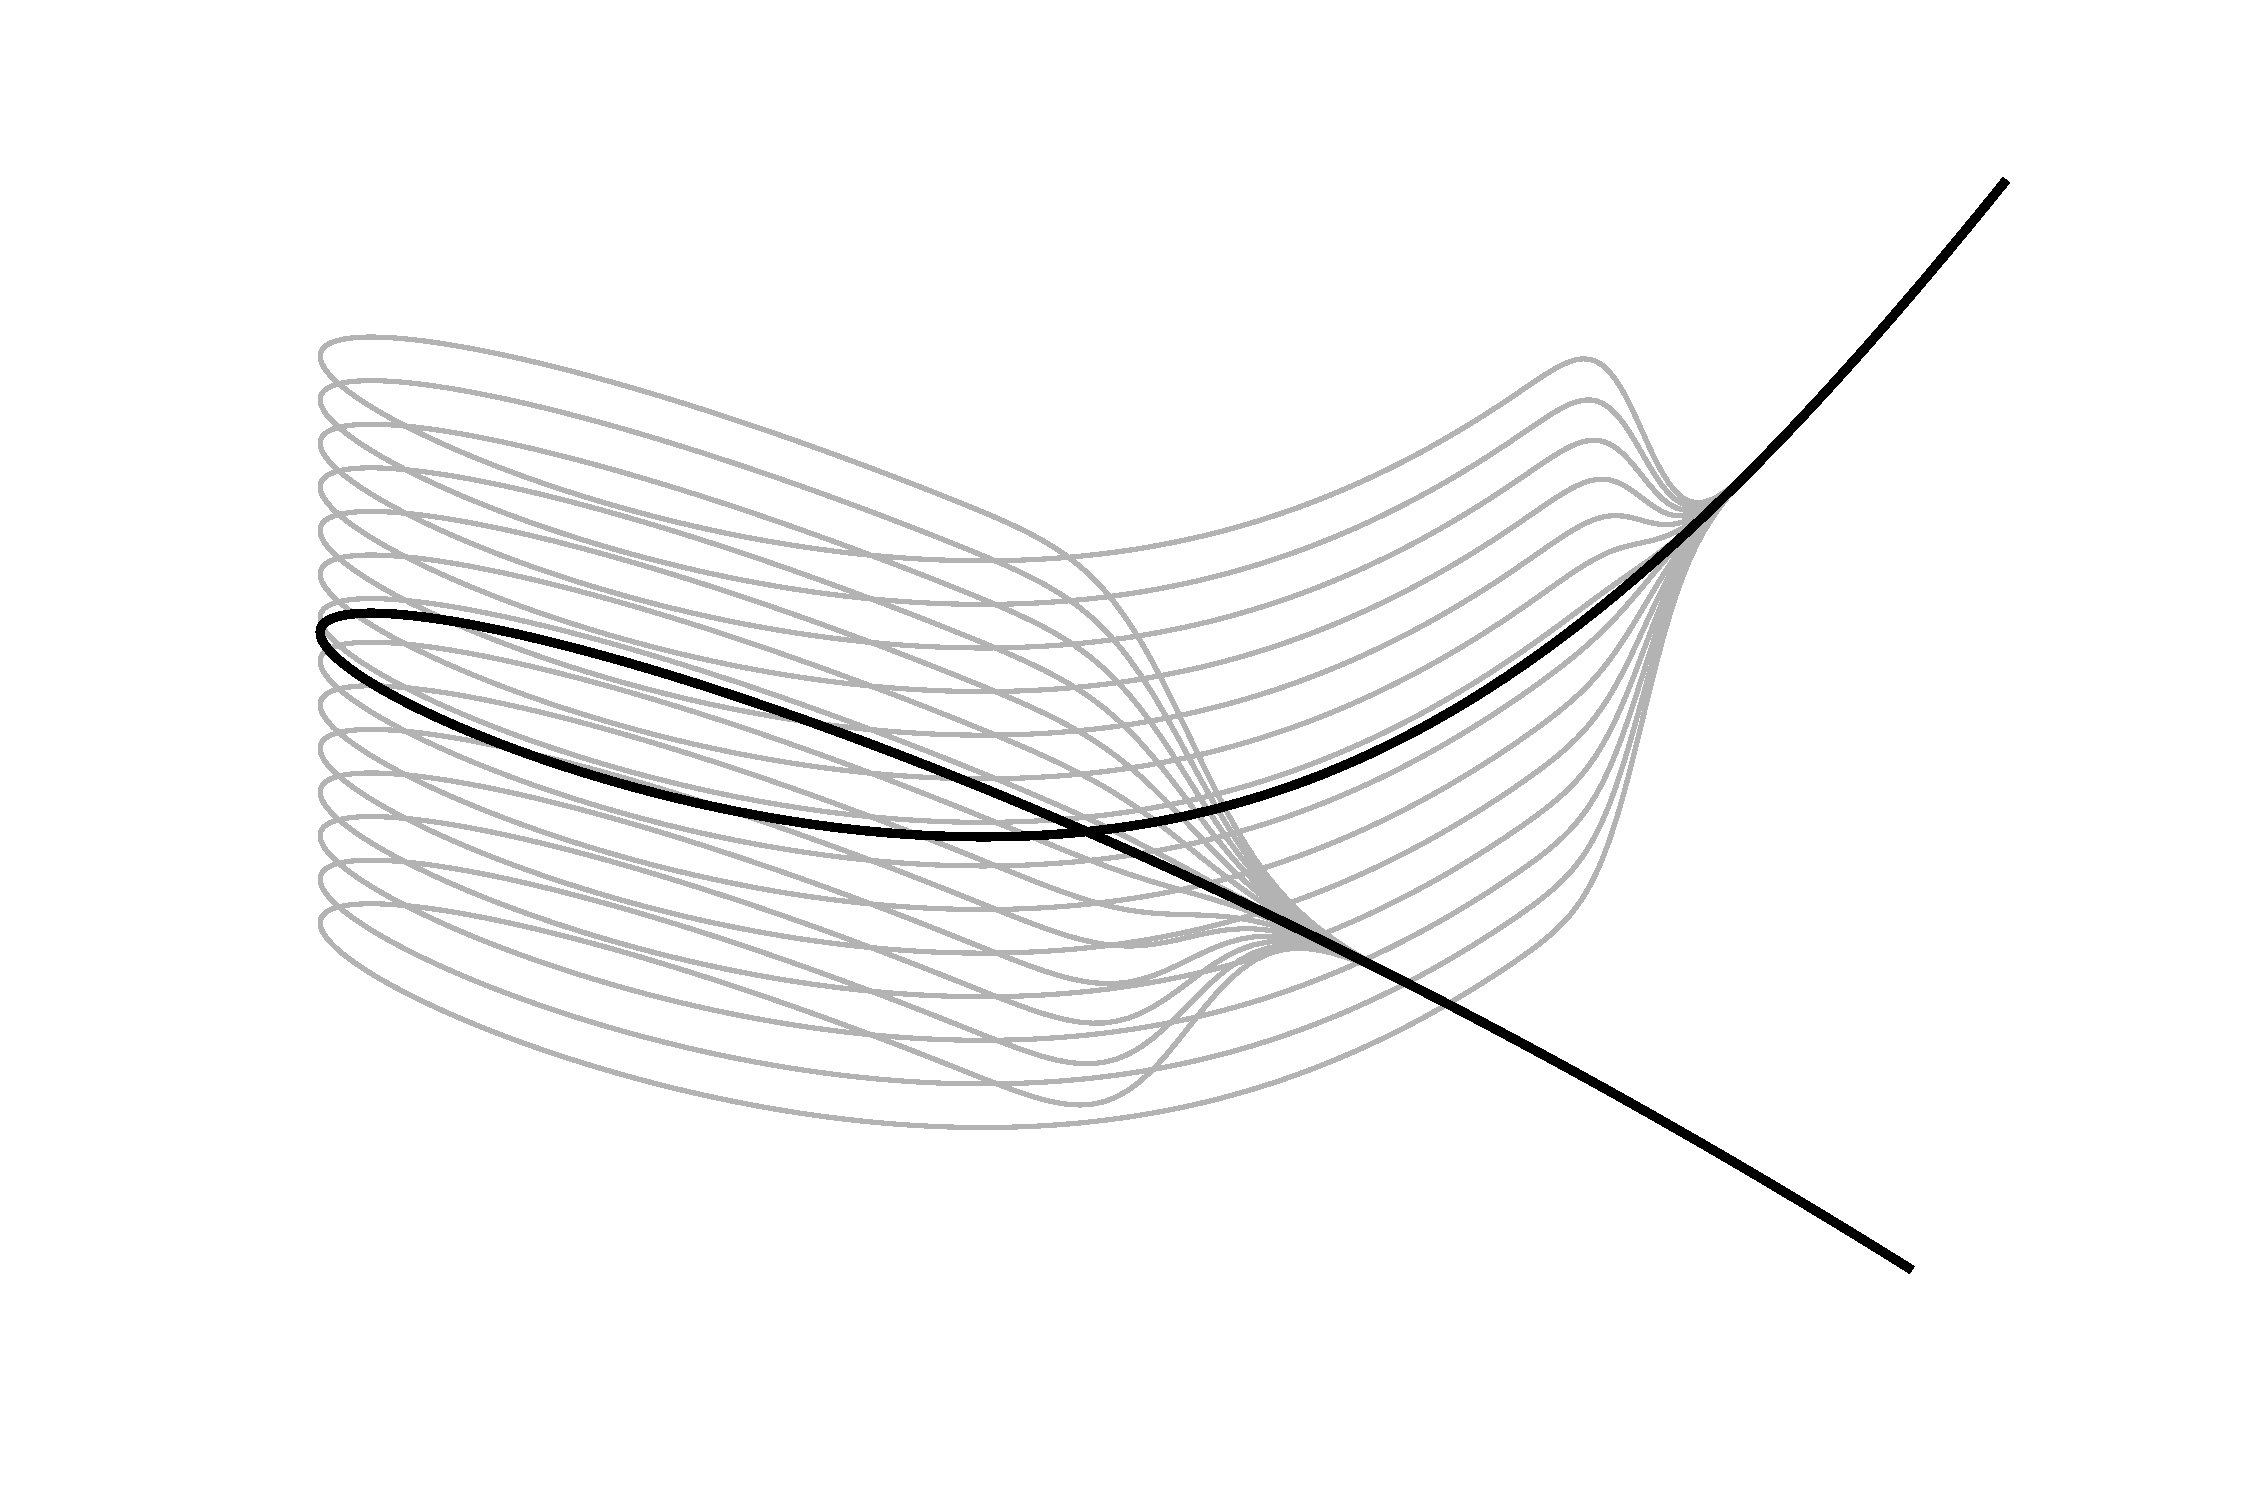
\includegraphics[width = .83\textwidth]{variation.pdf}
		\caption{Example of a variation of the path $\gamma(t) = (\gamma^1(t),\gamma^2(t))$ in $\mathbb{R}^2$ defined by $\gamma(t) := (t^2 + \sin(t)\cos(t),t^3 - t)$ for $t \in \intcc[0]{-\frac{3}{2},\frac{3}{2}}$ along the second coordinate using a smooth bump function as in \cite[42]{lee:smooth_manifolds:2013}.}
		\label{fig:variation}
	\end{figure}
\end{example}

\begin{exercise}
	\label{ex:U_delta_neighbourhood}
	Let $(X,d)$ be a metric space and $A \subseteq U \subseteq X$ where $U$ is open in $X$ and $A$ is closed in $X$. Then there exists $\delta > 0$ such that
	\begin{equation*}
		U_\delta := \cbr[0]{x \in X : \dist(x,A) < \delta} \subseteq U.
	\end{equation*}
\end{exercise}

\begin{definition}[Action Functional]
	Let $(M,L)$ be a Lagrangian system and $\mathcal{P}(M)$ be a path space. The morphism $S : \mathcal{P}(M) \to \mathbb{R}$ defined by
	\begin{equation*}
		S(\gamma) := \int_{t_0}^{t_1} L\del[0]{\gamma(t),\dot{\gamma}(t),t} dt
	\end{equation*}
	\noindent is called the \bld{action functional associated to the Lagrangian system $(M,L)$}\index{Action functional}.
\end{definition}

Motions of Lagrangian systems are characterized by an axiom.

\begin{axiom}[Hamilton's Principle of Least Action]\index{Hamilton!'s principle of least action}
	\label{ax:Hamilton_least_action}
	Let $(M,L)$ be a Lagrangian system and $\mathcal{P}(M)$ be a path space. A path $\gamma \in C^\infty(\intcc[0]{t_0,t_1},M)$ describes a motion of $(M,L)$ between $(x_0,t_0)$ and $(x_1,t_1)$ if and only if 
	\begin{equation}
		\frac{d}{d\varepsilon}\bigg\vert_{\varepsilon = 0} S(\gamma_\varepsilon) = 0
	\end{equation}
	\noindent for all variations $\gamma_\varepsilon$ of $\gamma$.
\end{axiom}

\begin{definition}[Extremal]
	A motion of a Lagrangian system between two points is called an \bld{extremal of the action functional $S$}\index{Extremal}.
\end{definition}

The Newton-Laplace determinacy principle \ref{ax:NL_determinacy_principle} implies that motions of mechanical systems can be described as solutions of second order ordinary differential equations. That this is indeed the case, is shown by the next theorem. But first, let us fix some notation. Let $M^n$ be a smooth manifold and $(U,\varphi)$ be a chart on $M$ with coordinates $(x^i)$. In what follows, we will use the abbreviation
\begin{equation*}
	\frac{\partial}{\partial x} := \del[3]{\frac{\partial}{\partial x^1},\dots,\frac{\partial}{\partial x^n}},
\end{equation*}
\noindent where as usual $\frac{\partial}{\partial x^i} : U \to TM$ denotes the \emph{$i$-th coordinate vector field}, that is
\begin{equation*}
	\frac{\partial f}{\partial x^i}(x) := \frac{\partial}{\partial x^i}\bigg\vert_x f = \partial_i(f \circ \varphi^{-1})\del[1]{\varphi(x)},
\end{equation*}
\noindent for all $i = 1,\dots,n$, $x \in U$ and $f \in C^\infty(M)$. Also recall, that on this chart
\begin{equation}
	\label{eq:differential_of_a_function}
	df_x = \frac{\partial f}{\partial x^i}(x)dx^i\vert_x
\end{equation}
\noindent holds for all $x \in U$ (see \cite[281]{lee:smooth_manifolds:2013}). Additionally, we need the following proposition.

\begin{proposition}[{Derivative of a Function along a Curve \cite[283]{lee:smooth_manifolds:2013}}]
	\label{prop:derivative_of_a_function_along_a_curve}
	Suppose $M$ is a smooth manifold, $J \subseteq \mathbb{R}$ an interval, $\gamma \in C^\infty(J,M)$ a curve on $M$ and $f \in C^\infty(M)$. Then for all $t \in J$ holds
	\begin{equation*}
		(f \circ \gamma)'(t) = df_{\gamma(t)}\del[1]{\gamma'(t)}.
	\end{equation*}
\end{proposition}

\begin{theorem}[Euler-Lagrange Equations]
	\label{thm:EL_equations}
	Let $(M^n,L)$ be a Lagrangian system. A path $\gamma \in C^\infty(\intcc[0]{t_0,t_1},M)$ describes a motion of $(M,L)$ between $(x_0,t_0)$ and $(x_1,t_1)$ if and only if with respect to all charts $(U,x^i)$
	\begin{equation}
		\label{eq:EL_equations}
		\pd{L}{x}\del[1]{\gamma(t),\dot{\gamma}(t),t} - \frac{d}{dt} \pd{L}{v}\del[1]{\gamma(t),\dot{\gamma}(t),t} = 0
	\end{equation}
	\noindent holds, where $(x^i,v^i)$ denotes the standard coordinates on $TM$. The system of equations \textup{(}\ref{eq:EL_equations}\textup{)} is referred to as the \bld{Euler-Lagrange equations}\index{Equations!Euler-Lagrange}.
\end{theorem}

\begin{proof}
	By Hamilton's principle of least action \ref{ax:Hamilton_least_action}, we may assume that $\gamma$ is an extremal of the action functional $S$. The proof is divided into two steps.\\
	\emph{Step 1: Suppose that $\gamma$ is contained in a chart domain $U$.} Let $t \in \intcc[0]{t_0,t_1}$ and abreviate $x_t := (\gamma(t),\dot{\gamma}(t),t)$. Suppose $\Gamma : \intcc[0]{t_0,t_1} \times \intcc[0]{-\varepsilon_0,\varepsilon_0} \to M$ is a variation of $\gamma$. Then there exists a rectangle $\mathcal{R}$ such that
	\begin{equation*}
		\intcc[0]{t_0,t_1} \times \cbr[0]{0} \subseteq \mathcal{R} \subseteq \intcc[0]{t_0,t_1} \times \intcc[0]{-\varepsilon_0,\varepsilon_0} 
	\end{equation*} 
	\noindent and $\Gamma(\mathcal{R}) \subseteq U$. Indeed, $\Gamma$ is continuous since $\Gamma$ is smooth and so $\Gamma^{-1}(U)$ is open in $\intcc[0]{t_0,t_1} \times \intcc[0]{-\varepsilon_0,\varepsilon_0}$. Since $\gamma$ is a path in $U$, we get
	\begin{equation*}
		\intcc[0]{t_0,t_1} \times \cbr{0} \subseteq \Gamma^{-1}(U)
	\end{equation*}
	\noindent by the definition of a variation. By exercise 2.4. (c) \cite[22]{lee:topological_manifolds:2011}, the standard Euclidean metric and the \emph{maximum metric $\abs{\>\cdot\>}_\infty$} generate the same topology, thus for all $t \in \intcc[0]{t_0,t_1}$ there exists $r_t > 0$ such that
	\begin{equation*}
		B_{r_t}(t,0) := \cbr[1]{(x,\varepsilon) \in \intcc[0]{t_0,t_1} \times \intcc[0]{-\varepsilon_0,\varepsilon_0} : \max\cbr[0]{\>\abs{x - t},\abs{\varepsilon}} < r_t} \subseteq \Gamma^{-1}(U).
	\end{equation*}
	Since $\intcc[0]{t_0,t_1} \times \cbr[0]{0}$ is compact in $\intcc[0]{t_0,t_1} \times \intcc[0]{-\varepsilon_0,\varepsilon_0}$, we find $m \in \mathbb{N}$ such that 
	\begin{equation*}
		\intcc[0]{t_0,t_1} \times \cbr[0]{0} \subseteq \bigcup_{i = 1}^m B_{r_i}(t_i,0).
	\end{equation*}
	Set $r := \max_{i = 1,\dots,m} r_i$ and define $\mathcal{R} := \intcc[0]{t_0,t_1} \times \intoo[0]{-r,r}$. Then if $(t,\varepsilon) \in \mathcal{R}$ we get that there exists some index $i$ such that $(t,0) \in B_{r_i}(t_i,0)$. Hence $\abs{t - t_i} < r_i$ and so
	\begin{equation*}
		\abs[0]{(t,\varepsilon) - (t_i,0)}_\infty = \max\cbr[0]{\> \abs{t - t_i},\abs{\varepsilon}} < r_i.
	\end{equation*}
	Thus $(t,\varepsilon) \subseteq B_{r_i}(t_i,0) \subseteq \Gamma^{-1}(U)$ and so $\Gamma(\mathcal{R}) \subseteq U$. Hence we can write
	\begin{equation*}
		\gamma_\varepsilon(t) = \del[1]{\gamma_\varepsilon^1(t),\dots,\gamma_\varepsilon^n(t)}
	\end{equation*}
	\noindent and 
	\begin{equation*}
		\dot{\gamma}_\varepsilon(t) = \del[1]{\dot{\gamma}_\varepsilon^1(t),\dots,\dot{\gamma}_\varepsilon^n(t)}
	\end{equation*}
	\noindent for all $(x,\varepsilon) \in \mathcal{R}$, where the dot denotes a derivative with respect to time.\\
	Using the formula for the derivative of a function along a curve \ref{prop:derivative_of_a_function_along_a_curve}, we compute
	\begin{align*}
		\frac{d}{d\varepsilon}\bigg\vert_{\varepsilon = 0} L\del[1]{\gamma_\varepsilon(t),\dot{\gamma}_\varepsilon(t),t} &= dL_{x_t}\del[3]{\frac{d}{d\varepsilon}\bigg\vert_{\varepsilon = 0}\gamma_\varepsilon(t),\frac{d}{d\varepsilon}\bigg\vert_{\varepsilon = 0}\dot{\gamma}_\varepsilon(t),0}\\
		&= dL_{x_t}\del[3]{\frac{d\gamma_\varepsilon^j(t)}{d\varepsilon}(0)\frac{\partial}{\partial x^j}\bigg\vert_{\gamma(t)},\frac{d\dot{\gamma}_\varepsilon^j(t)}{d\varepsilon}(0)\frac{\partial}{\partial v^j}\bigg\vert_{\dot{\gamma}(t)},0}.
	\end{align*}
	\noindent for all variations $\gamma_\varepsilon$ of $\gamma$ in $U$. Moreover, using the formula for the differential of a function on coordinates (\ref{eq:differential_of_a_function}) yields
	\begin{equation*}
		dL_{x_t} = \frac{\partial L}{\partial x^i}(x_t) dx^i\vert_{x_t} + \frac{\partial L}{\partial v^i}(x_t) dv^i\vert_{x_t} + \frac{\partial L}{\partial t}(x_t)dt\vert_{x_t}.
	\end{equation*}
	Therefore
	\begin{align*}
		0 &= \frac{d}{d\varepsilon}\bigg\vert_{\varepsilon = 0} S(\gamma_\varepsilon)\\
		&= \int_{t_0}^{t_1} \frac{d}{d\varepsilon}\bigg\vert_{\varepsilon = 0} L\del[1]{\gamma_\varepsilon(t),\dot{\gamma}_\varepsilon(t),t} dt\\
		&= \int_{t_0}^{t_1} dL_{x_t}\del[3]{\frac{d\gamma_\varepsilon^j(t)}{d\varepsilon}(0)\frac{\partial}{\partial x^j}\bigg\vert_{\gamma(t)},\frac{d\dot{\gamma}_\varepsilon^j(t)}{d\varepsilon}(0)\frac{\partial}{\partial v^j}\bigg\vert_{\dot{\gamma}(t)},0}\\
		&= \int_{t_0}^{t_1} \frac{\partial L}{\partial x^i}(x_t)\frac{d\gamma_\varepsilon^i(t)}{d\varepsilon}(0)dt + \int_{t_0}^{t_1}\frac{\partial L}{\partial v^i}(x_t)\frac{d\dot{\gamma}_\varepsilon^i(t)}{d\varepsilon}(0)dt\\
		&= \int_{t_0}^{t_1} \frac{\partial L}{\partial x^i}(x_t)\frac{d\gamma_\varepsilon^i(t)}{d\varepsilon}(0)dt + \int_{t_0}^{t_1}\frac{\partial L}{\partial v^i}(x_t)\del[3]{\frac{d\gamma_\varepsilon^i(t)}{d\varepsilon}(0)}'dt\\
		&= \int_{t_0}^{t_1} \frac{\partial L}{\partial x^i}(x_t)\frac{d\gamma_\varepsilon^i(t)}{d\varepsilon}(0)dt + \frac{\partial L}{\partial v^i}(x_t)\frac{d\gamma_\varepsilon^i(t)}{d\varepsilon}(0)\bigg\vert_{t_0}^{t_1} - \int_{t_0}^{t_1} \frac{d}{dt}\frac{\partial L}{\partial v^i}(x_t)\frac{d\gamma_\varepsilon^i(t)}{d\varepsilon}(0)dt\\
		&= \int_{t_0}^{t_1} \del[3]{\frac{\partial L}{\partial x^i}(x_t) - \frac{d}{dt}\frac{\partial L}{\partial v^i}(x_t)}\frac{d\gamma_\varepsilon^i(t)}{d\varepsilon}(0)dt 
	\end{align*}
	\noindent since $\gamma^i_\varepsilon(t_0)$ and $\gamma^i_\varepsilon(t_1)$ are constant by definition of a variation. Let $f \in C^\infty_c\intoo[0]{t_0,t_1}$, $j = 1,\dots,n$ and $\gamma_\varepsilon$ be the variation of $\gamma$ defined in example \ref{ex:perturbation_along_single_direction} along the $j$-th direction. Above computation therefore yields
	\begin{equation*}
		0 = \int_{t_0}^{t_1} \del[3]{\frac{\partial L}{\partial x^j}(x_t) - \frac{d}{dt}\frac{\partial L}{\partial v^j}(x_t)}f(t) dt
	\end{equation*}
	\noindent for all $f \in C^\infty_c\intoo[0]{t_0,t_1}$. Hence the fundamental lemma of calculus of variations \ref{lem:fundamental_lemma} implies
	\begin{equation*}
		\frac{\partial L}{\partial x^j}(x_t) - \frac{d}{dt}\frac{\partial L}{\partial v^j}(x_t) = 0
	\end{equation*}
	\noindent for all $j = 1,\dots,n$.\\
	Conversly, if we assume that the Euler-Lagrange equations (\ref{eq:EL_equations}) hold, above computation yields
	\begin{equation*}
		\frac{d}{d\varepsilon}\bigg\vert_{\varepsilon = 0} S(\gamma_\varepsilon) = \int_{t_0}^{t_1} \del[3]{\frac{\partial L}{\partial x^i}(x_t) - \frac{d}{dt}\frac{\partial L}{\partial v^i}(x_t)}\frac{d\gamma_\varepsilon^i(t)}{d\varepsilon}(0)dt = 0
	\end{equation*}
	\noindent for every variation $\gamma_\varepsilon$ of $\gamma$.\\
	\emph{Step 2: Suppose that $\gamma$ is an arbitrary extremal of $S$.} The key technical result used here is the following lemma.
	\begin{lemma}[{Lebesgue Number Lemma \cite[194]{lee:topological_manifolds:2011}}]
		\label{lem:Lebesgue_number_lemma}
		Every open cover of a compact metric space admits a Lebesgue number, i.e. a number $\delta > 0$ such that every subset of the metric space with diameter less than $\delta$ is contained in a member of the family.
	\end{lemma}
	Let $(U_\alpha)_{\alpha \in A}$ be the smooth structure on $M$, i.e. the maximal smooth atlas. Since $\gamma$ is continuous, $\del[1]{\gamma^{-1}(U_\alpha)}_{\alpha \in A}$ is an open cover for $\intcc[0]{t_0,t_1}$. By the Lebesgue number lemma \ref{lem:Lebesgue_number_lemma}, this open cover admits a Lebesgue number $\delta > 0$. Let $N \in \mathbb{N}$ such that $(t_1 - t_0)/N < \delta$ and define
	\begin{equation*}
		t_i := \frac{i}{N}(t_1 - t_0) + t_0
	\end{equation*}
	\noindent for all $i = 0,\dots,N$. Then for all $i = 1,\dots,N$, $\gamma\vert_{\intcc[0]{t_{i - 1},t_i}}$ is contained in $U_\alpha$ for some $\alpha \in A$. Let us extend the construction of example \ref{ex:perturbation_along_single_direction}. Suppose $f \in C^\infty_c(t_{i - 1},t_i)$. Then we can define a variation $\Gamma : \intcc[0]{t_0,t_1} \times \intcc[0]{-\varepsilon_0,\varepsilon_0} \to M$ as follows: Define 
	\begin{equation*}
		\Gamma : \del[0]{\intcc[0]{t_0,t_1}\setminus \supp f} \times \intcc[0]{-\varepsilon_0,\varepsilon_0} \to M
	\end{equation*}
	\noindent by $\Gamma(t,\varepsilon) := \gamma(t)$, and $\Gamma : \intoo[0]{t_{i - 1},t_i} \times \intcc[0]{-\varepsilon_0,\varepsilon_0} \to M$ to be the map defined in example \ref{ex:perturbation_along_single_direction}. Since both definitions agree on the overlap $\intoo[0]{t_{i - 1},t_i} \setminus \supp f$, an application of the gluing lemma for smooth maps \cite[35]{lee:smooth_manifolds:2013} yields the existence of a variation $\Gamma$ of $\gamma$ on $M$.
	Therefore, step 1 implies the Euler-Lagrange equations (\ref{eq:EL_equations}). The converse direction is content of problem \ref{prob:1-1.}
\end{proof}

Due to the Newton-Laplace Determinacy Principle \ref{ax:NL_determinacy_principle}, the motions on a Lagrangian system are inherently characterized by the Lagrangian function and locally by the Euler-Lagrange equations (\ref{eq:EL_equations}). Hence any motion satisfies locally a system of second order ordinary differential equations. This system bears its own name.

\begin{definition}[Equations of Motion]
	The Euler-Lagrange equations \textup{(}\ref{eq:EL_equations}\textup{)} of a Lagrangian system are called the \bld{equations of motion}\index{Equations!of motion}.
\end{definition}

\begin{example}[Motions on Riemannian Manifolds]
	\label{ex:motions_on_Riemannian_manifolds}
	Let $(M^n,g)$ be a Riemannian manifold and consider the Lagrangian $L$ on $M$ defined in example \ref{ex:Lagrangian} with kinetic energy
	\begin{equation*}
		T(x,v,t) := \frac{1}{2}g_x(v,v) = \frac{1}{2}\abs{v}^2_g
	\end{equation*}
	\noindent and potential energy $V(x,t) := 0$ for $x \in M$, $v \in T_xM$ and $t \in \mathbb{R}$. Let $(U,x^i)$ be a chart on $M$. We compute
	\begin{align*}
		L(x,v,t) &= \frac{1}{2}g_{x}\del[0]{v,v}\\
		&= \frac{1}{2}g_{x}\del[3]{v^i\frac{\partial}{\partial x^i}\bigg\vert_x,v^j\frac{\partial}{\partial x^j}\bigg\vert_x}\\
		&= \frac{1}{2}g_{x}\del[3]{\frac{\partial}{\partial x^i}\bigg\vert_x,\frac{\partial}{\partial x^j}\bigg\vert_x}v^iv^j\\
		&= \frac{1}{2}g_{ij}(x)v^iv^j,
	\end{align*}
	\noindent where $g_{ij}(x) := g_{x}\del[1]{\frac{\partial}{\partial x^i}\big\vert_x,\frac{\partial}{\partial x^j}\big\vert_x}$. Thus 
	\begin{equation*}
		\frac{\partial L}{\partial x^l}(x,v,t) = \frac{1}{2}\frac{\partial g_{ij}}{\partial x^l}(x)v^i v^j
	\end{equation*}
	\noindent and in particular
	\begin{equation*}
		\frac{\partial L}{\partial x^l}\del[1]{\gamma(t),\dot{\gamma}(t),t} = \frac{1}{2}\frac{\partial g_{ij}}{\partial x^l}\del[1]{\gamma(t)}\dot{\gamma}^i(t) \dot{\gamma}^j(t),
	\end{equation*}
	\noindent for all $l = 1,\dots,n$. Moreover
	\begin{equation*}
		\frac{\partial L}{\partial v^l}(x,v,t) = \frac{1}{2}g_{ij}(x)\delta^i_lv^j + \frac{1}{2}g_{ij}(x)v^i\delta^j_l = \frac{1}{2}g_{lj}(x)v^j + \frac{1}{2}g_{il}(x)v^i
	\end{equation*}
	\noindent implies
	\begin{align*}
		\frac{d}{dt}\frac{\partial L}{\partial v^l}\del[1]{\gamma(t),\dot{\gamma}(t),t} &= \frac{1}{2}\frac{d}{dt}g_{lj}(\gamma)\dot{\gamma}^j + \frac{1}{2}g_{lj}(\gamma)\ddot{\gamma}^j + \frac{1}{2}\frac{d}{dt}g_{il}(\gamma)\dot{\gamma}^i + \frac{1}{2}g_{il}(\gamma)\ddot{\gamma}^i\\
		&= \frac{1}{2}dg_{lj}(\dot{\gamma})\dot{\gamma}^j + \frac{1}{2}g_{lj}(\gamma)\ddot{\gamma}^j + \frac{1}{2}dg_{il}(\dot{\gamma})\dot{\gamma}^i + \frac{1}{2}g_{il}(\gamma)\ddot{\gamma}^i\\
		&= \frac{1}{2}\frac{\partial g_{lj}}{\partial x^k}\dot{\gamma}^k\dot{\gamma}^j + \frac{1}{2}g_{lj}(\gamma)\ddot{\gamma}^j + \frac{1}{2}\frac{\partial g_{il}}{\partial x^k}\dot{\gamma}^k\dot{\gamma}^i + \frac{1}{2}g_{il}(\gamma)\ddot{\gamma}^i\\
		&= \frac{1}{2}\frac{\partial g_{jl}}{\partial x^k}\dot{\gamma}^k\dot{\gamma}^j + \frac{1}{2}g_{jl}(\gamma)\ddot{\gamma}^j + \frac{1}{2}\frac{\partial g_{il}}{\partial x^k}\dot{\gamma}^k\dot{\gamma}^i + \frac{1}{2}g_{il}(\gamma)\ddot{\gamma}^i\\
		&= g_{il}\ddot{\gamma}^i + \frac{1}{2}\frac{\partial g_{jl}}{\partial x^i}\dot{\gamma}^i\dot{\gamma}^j + \frac{1}{2}\frac{\partial g_{il}}{\partial x^j}\dot{\gamma}^i\dot{\gamma}^j.
	\end{align*}
	Therefore the Euler-Lagrange equations (\ref{eq:EL_equations}) read
	\begin{equation*}
		0 = \frac{d}{dt}\frac{\partial L}{\partial v^l} - \frac{\partial L}{\partial x^l} = g_{il}\ddot{\gamma}^i + \frac{1}{2}\del[3]{\frac{\partial g_{jl}}{\partial x^i} + \frac{\partial g_{il}}{\partial x^j} - \frac{\partial g_{ij}}{\partial x^l}}\dot{\gamma}^i\dot{\gamma}^j,	
	\end{equation*}
	\noindent for all $l = 1,\dots,n$. Multiplying both sides by $g^{kl}$ yields
	\begin{equation}
		\label{eq:geodesic_equation}
		\ddot{\gamma}^k + \Gamma^k_{ij}\dot{\gamma}^i \dot{\gamma}^j = 0,
	\end{equation}
	\noindent for all $k = 1,\dots,n$, where
	\begin{equation*}
		\Gamma^k_{ij} := \frac{1}{2}g^{kl}\del[3]{\frac{\partial g_{jl}}{\partial x^i} + \frac{\partial g_{il}}{\partial x^j} - \frac{\partial g_{ij}}{\partial x^l}}
	\end{equation*}
	\noindent are the \bld{Christoffel symbols}\index{Symbols!Christoffel} with respect to the choosen chart (see \cite[70]{lee:Riemannian_manifolds:1997}). The system of equations (\ref{eq:geodesic_equation}) is called \bld{geodesic equations}\index{Equations!geodesic} (see \cite[58]{lee:Riemannian_manifolds:1997}). Hence extremals $\gamma$ of the action functional satisfy the geodesic equation and are therefore geodesics on the Riemannian manifold $M$.
\end{example}

\begin{lemma}
	\label{lem:same_equations_of_motion}
	Let $(M,L)$ be a Lagrangian system and define $L + df \in C^\infty(TM \times \mathbb{R})$ by
	\begin{equation*}
		(L + df)(x,v,t) := L(x,v,t) + df_x(v)
	\end{equation*}
	\noindent for any $f \in C^\infty(M)$. Then $(M,L)$ and $(M,L + df)$ admit the same equations of motion.
\end{lemma}

\begin{proof}
	Let us denote the action function corresponding to $L + df$ by $\wtilde{S}$ and suppose $\gamma_\varepsilon$ is a variation of $\gamma$ in $M$. Using the formula for the derivative of a function along a curve \cite[283]{lee:smooth_manifolds:2013} we compute
	\begin{align*}
		\wtilde{S}(\gamma_\varepsilon) &= \int_{t_0}^{t_1}L(\gamma_\varepsilon(t),\dot{\gamma}_\varepsilon(t),t)dt + \int_{t_0}^{t_1}df_{\gamma_\varepsilon(t)}\del[1]{\dot{\gamma}_\varepsilon(t)}dt\\
		&= S(\gamma_\varepsilon) + \int_{t_0}^{t_1}(f \circ \gamma_\varepsilon)'(t)dt\\
		&= S(\gamma_\varepsilon) + f\del[1]{\gamma_\varepsilon(t_1)} - f\del[1]{\gamma_{\varepsilon}(t_0)}\\
		&= S(\gamma_\varepsilon) + f(x_1) - f(x_0).
	\end{align*}
	In particular
	\begin{equation*}
		\frac{d}{d\varepsilon}\bigg\vert_{\varepsilon = 0}\wtilde{S}(\gamma_\varepsilon) = \frac{d}{d\varepsilon}\bigg\vert_{\varepsilon = 0}S(\gamma_\varepsilon).
	\end{equation*}
\end{proof}

\begin{remark}
	Lemma \ref{lem:same_equations_of_motion} implies, that the Lagrangian of a mechanical system can only be determined up to differentials of smooth functions. Actually, in coordinates, also up to total time derivatives. Hence a \emph{law of motion}, that is a Lagrangian describing a certain mechanical system, is in fact an equivalence class of Lagrangian functions.
\end{remark}

\section*{Legendre Transform}
In this section we \emph{dualize} the notion of a Lagrangian function, that is, to each Lagrangian function $L \in C^\infty(TM)$ we will associate a \emph{dual function} $L^* \in C^\infty(T^*M)$. It turns out, that in this dual formulation, the equations of motion take a very symmetric form. To simplify the notation and illuminating the main concept, we consider Lagrangian functions of a special type.

\begin{definition}[Autonomous System]
	A Lagrangian system $(M,L)$ is said to be an \bld{autonomous Lagrangian system}\index{Lagrangian!system!autonomous}, iff $L \in C^\infty(TM)$.
\end{definition}

Let $(M^n,L)$ be an autonomous Lagrangian system and $(U,x^i)$ a chart on $M$. Moreover, let $(x^i,v^i)$ denote standard coordinates on $TM$, that is $v^i := dx^i$ for all $i = 1,\dots,n$. Expanding the Euler-Lagrange equations (\ref{eq:EL_equations}) yields
\begin{align*}
	\frac{\partial L}{\partial x^j}\del[1]{\gamma(t),\dot{\gamma}(t)} &= \frac{d}{dt}\frac{\partial L}{\partial v^j}\del[1]{\gamma(t),\dot{\gamma}(t)}\\
	&= \frac{\partial^2 L}{\partial x^i\partial v^j}\del[1]{\gamma(t),\dot{\gamma}(t)}\dot{\gamma}^i(t) + \frac{\partial^2 L}{\partial v^i\partial v^j}\del[1]{\gamma(t),\dot{\gamma}(t)}\ddot{\gamma}^i(t)
\end{align*}
\noindent for all $j = 1,\dots,n$. In order to solve above system of second order ordinary differential equations for $\ddot{\gamma}^i(t)$ and all initial conditions in the chart on $TU$, the matrix $\mathcal{H}_L(x,v)$ defined by
\begin{equation}
	\label{eq:H_L}
	\mathcal{H}_L(x,v) := \del[3]{\frac{\partial^2 L}{\partial v^i\partial v^j}(x,v)}_j^i
\end{equation}
\noindent must be invertible on $TU$.

\begin{definition}[Nondegenrate System]
	An autonomous Lagrangian system $(M,L)$ is said to be \bld{nondegenerate}\index{Lagrangian!system!nondegenerate}, iff for all coordinate charts $U$ on $M$, $\det \mathcal{H}_L(x,v) \neq 0$ holds on $TU$. 
\end{definition}

\begin{example}[Nondegenrate System on a Riemannian Manifold]
	\label{ex:nondegenerate_Lagrangian_system}
	Let $(M,g)$ be a Riemannian manifold. Consider the Lagrangian $T - V$ with kinetic energy $T \in C^\infty(TM)$ defined by $T(v) := \frac{1}{2}\abs{v}^2$ and potential energy $V \in C^\infty(M)$. Then the computation performed in example \ref{ex:motions_on_Riemannian_manifolds} yields
	\begin{equation*}
		\mathcal{H}_{T - V}(x,v) = \del[1]{g_{ij}(x)}^i_j
	\end{equation*} 
	\noindent on every chart since $\frac{\partial V}{\partial v^i} = 0$ for every $i$, and so this Lagrangian system is nondegenerate.
\end{example}

The nondegeneracy of an autonomous Lagrangian system is intrinsically connected to a certain differential form in $\Omega^1(TM)$, which we will construct now. For every $(x,v) \in TM$ we can define a covector $D^\mathcal{F}_{(x,v)} L \in T^*_xM$ by setting
\begin{equation}
	D^\mathcal{F}_{(x,v)}L := \frac{\partial}{\partial v^i}\bigg\vert_{(x,v)}(L) dx^i\vert_x = \frac{\partial L}{\partial v^i}dx^i.
\end{equation}
Let $(\wtilde{U},\wtilde{x}^i)$ be another chart on $M$ such that $U \cap \wtilde{U} \neq \varnothing$. Denote the induced coordinates on $TM$ by $(\wtilde{x}^i,\wtilde{v}^i)$. Then on $U \cap \wtilde{U}$ we have that 
\begin{equation*}
	\frac{\partial}{\partial \wtilde{v}^i} = \frac{\partial x^j}{\partial \wtilde{v}^i}\frac{\partial}{\partial x^j} + \frac{\partial v^j}{\partial \wtilde{v}^i}\frac{\partial}{\partial v^j} = \frac{\partial v^j}{\partial \wtilde{v}^i}\frac{\partial}{\partial v^j}.
\end{equation*}
Moreover
\begin{equation*}
	\frac{\partial}{\partial x^j} = \frac{\partial \wtilde{x}^k}{\partial x^j} \frac{\partial}{\partial \wtilde{x}^k}
\end{equation*}
\noindent which implies
\begin{equation*}
	d\wtilde{x}^i \del[3]{\frac{\partial}{\partial x^j}} = \frac{\partial \wtilde{x}^k}{\partial x^j} d\wtilde{x}^i\del[3]{\frac{\partial}{\partial \wtilde{x}^k}} = \frac{\partial \wtilde{x}^k}{\partial x^j}\delta^i_k = \frac{\partial \wtilde{x}^i}{\partial x^j}.
\end{equation*}
Thus
\begin{equation*}
	d\wtilde{x}^i = \frac{\partial \wtilde{x}^i}{\partial x^j} dx^j
\end{equation*}
\noindent or equivalently 
\begin{equation*}
	v^j = \frac{\partial x^j}{\partial \wtilde{x}^i}\wtilde{v}^i,
\end{equation*}
\noindent and so we compute
\begin{equation*}
	D^\mathcal{F}L = \frac{\partial L}{\partial \wtilde{v}^i}d\wtilde{x}^i = \frac{\partial v^j}{\partial \wtilde{v}^i}\frac{\partial L}{\partial v^j}\frac{\partial \wtilde{x}^i}{\partial x^k} dx^k = \frac{\partial x^j}{\partial \wtilde{x}^i}\frac{\partial L}{\partial v^j}\frac{\partial \wtilde{x}^i}{\partial x^k} dx^k = \frac{\partial L}{\partial v^j}\delta^j_k dx^k = \frac{\partial L}{\partial v^j}dx^j.
\end{equation*}
Therefore, $D^\mathcal{F}L$ is independent of the choice of coordinates.

\begin{definition}[Fibrewise Differential\footnote{\unboldmath This terminology is adapted from exercise C.3. on problem sheet C of the lecture \emph{Differential geometry I} taught by \emph{Will J. Merry} at \emph{ETH Z\"urich} in the autumn semester $2018$, which can be found \href{https://www.merry.io/differential-geometry-i-problem-sheets/problem-sheet-c}{here}. See also \cite[2]{mazzucchelli:CPT:2012}.}]
	\label{def:fibrewise_differential}
	Let $(M,L)$ be an autonomous Lagrangian system. The form $D^\mathcal{F}L \in \Omega^1(TM)$ defined on a chart $(U,x^i)$ of $M$ by
	\begin{equation}
		\label{eq:fibrewise_differential}
		D^\mathcal{F}L := \frac{\partial L}{\partial v^i}dx^i
	\end{equation}
	\noindent where $(x^i,v^i)$ denotes the induced standard coordinates on $TM$, is called the \bld{fibrewise differential of $L$}\index{Differential!fibrewise}.
\end{definition}

\begin{remark}
	The preceeding discussion showed, that the fibrewise differential $D^\mathcal{F}L$ is well-defined.
\end{remark}

\begin{example}[Fibrewise Differential on a Riemannian Manifold]
	\label{ex:fibrewise_differential_Riemannian_manifold}
	Consider the autonomous Lagrangian system as defined in example \ref{ex:nondegenerate_Lagrangian_system}. Then the computation performed in example \ref{ex:motions_on_Riemannian_manifolds} yields
	\begin{equation*}
		D_{(x,v)}^\mathcal{F}(T - V) = g_{ij}(x)v^idx^j
	\end{equation*}
	\noindent on every chart since $\frac{\partial V}{\partial v^j} = 0$ for all $j$.
\end{example}

Recall, that a $2$-covector on a finite-dimensional real vector space is said to be \emph{nondegenrate}, iff the matrix representation with respect to some basis is invertible. Moreover, a \emph{nondegenerate $2$-form} on a smooth manifold $M$ is defined to be a $2$-form $\omega$, such that $\omega_x$ is a nondegenrate $2$-covector for all $x \in M$ (see \cite[565,567]{lee:smooth_manifolds:2013}). 

\begin{proposition}
	An autonomous Lagrangian system $(M,L)$ is nondegenerate if and only if $d(D^\mathcal{F}L)$ is nondegenerate.
\end{proposition}

\begin{proof}
	Using the computation performed in \cite[363]{lee:smooth_manifolds:2013}, we get
	\begin{equation*}
		d(D^\mathcal{F}L) = d\del[3]{\frac{\partial L}{\partial v^j}dx^j} = \frac{\partial^2 L}{\partial x^i\partial v^j}dx^i \wedge dx^j + \frac{\partial^2L}{\partial v^i\partial v^j}dv^i \wedge dx^j.
	\end{equation*}
	Moreover, using part (e) of properties of the wedge product \cite[356]{lee:smooth_manifolds:2013}, we compute
	\begin{align*}
		d(D^\mathcal{F}L)\del[3]{\frac{\partial}{\partial x^k},\frac{\partial}{\partial x^l}} =& \frac{\partial^2 L}{\partial x^i\partial v^j}\det\begin{pmatrix}
			\displaystyle dx^i\del[3]{\frac{\partial}{\partial x^k}} & \displaystyle dx^j\del[3]{\frac{\partial}{\partial x^k}}\\[4mm]
			\displaystyle dx^i\del[3]{\frac{\partial}{\partial x^l}} & \displaystyle dx^j\del[3]{\frac{\partial}{\partial x^l}}
		\end{pmatrix}\\ 
		&+ \frac{\partial^2L}{\partial v^i\partial v^j}\det\begin{pmatrix}
			\displaystyle dv^i\del[3]{\frac{\partial}{\partial x^k}} & \displaystyle dx^j\del[3]{\frac{\partial}{\partial x^k}}\\[4mm]
			\displaystyle dv^i\del[3]{\frac{\partial}{\partial x^l}} & \displaystyle dx^j\del[3]{\frac{\partial}{\partial x^l}}
		\end{pmatrix}\\
		=& \frac{\partial^2 L}{\partial x^i\partial v^j}(\delta^i_k\delta^j_l - \delta^i_l\delta^j_k)\\
		=& \frac{\partial^2 L}{\partial x^k\partial v^l} - \frac{\partial^2 L}{\partial x^l\partial v^k}
	\end{align*}
	\noindent for all $k,l = 1,\dots,n$. Similarly, we compute
	\begin{equation*}
		d(D^\mathcal{F}L)\del[3]{\frac{\partial}{\partial v^k},\frac{\partial}{\partial x^l}} = \frac{\partial^2 L}{\partial v^k\partial v^l} \qquad \text{and} \qquad d(D^\mathcal{F}L)\del[3]{\frac{\partial}{\partial v^k},\frac{\partial}{\partial v^l}} = 0,
	\end{equation*}
	\noindent and using skew-symmetry, we also deduce
	\begin{equation*}
		d(D^\mathcal{F}L)\del[3]{\frac{\partial}{\partial x^k},\frac{\partial}{\partial v^l}} = -\frac{\partial^2 L}{\partial v^k\partial v^l}.
	\end{equation*}
	Therefore, the matrix representing $d(D^\mathcal{F}L)$ with respect to the standard basis is given by the block matrix
	\begin{equation*}
		d(D^\mathcal{F}L) = \del{\begin{array}{c|c}
			* & -\mathcal{H}_L\\\hline
			\mathcal{H}_L & 0
		\end{array}},
	\end{equation*}
	\noindent where $\mathcal{H}_L$ is the matrix defined in (\ref{eq:H_L}). Thus 
	\begin{equation*}
		\det\del[1]{d(D^\mathcal{F}L)} = (-1)^n(\det \mathcal{H}_L)^2
	\end{equation*}
	Hence the matrix representation of $d(D^\mathcal{F}L)$ is invertible if and only if $\mathcal{H}_L$ is invertible, and the conclusion follows.
\end{proof}

So far, we have associated to each Lagrangian system $(M,L)$ a $1$-form on $TM$, the fibrewise differential $D^\mathcal{F}L$. In order to get closer to our goal of dualizing the concept of a Lagrangian function, we need also a $1$-form on $T^*M$. Suppose $(U,x^i)$ is a chart on $M$. The induced standard coordinates on the cotangent bundle $T^*M$ of $M$ are given by $(x^i,\xi_i)$, where $\xi_i := \frac{\partial}{\partial x^i}$, considered as an element of the double dual $T^{**}U$. On this chart, define a one $1$-form $\alpha$ by $\alpha := \xi_i dx^i$. Suppose $(\wtilde{x}^i,\wtilde{\xi}_i)$ are other coordinates. Then from the computations performed at the beginning of the previous section, we have that
\begin{equation*}
	\wtilde{\xi}_i = \frac{\partial x^j}{\partial \wtilde{x}^i}\xi_j \qquad \text{and} \qquad d\wtilde{x}^i = \frac{\partial \wtilde{x}^i}{\partial x^k}dx^k.
\end{equation*}
Thus
\begin{equation*}
	\alpha = \wtilde{\xi}_i d\wtilde{x}^i = \frac{\partial x^j}{\partial \wtilde{x}^i}\xi_j\frac{\partial \wtilde{x}^i}{\partial x^k}dx^k = \xi_j \delta^j_k dx^k = \xi_j dx^j,
\end{equation*}
\noindent and so, $\alpha$ is independen of the choice of coordinates.

\begin{definition}[Tautological Form]
	\label{def:tautological_form}
	Let $M$ be a smooth manifold. The \bld{tautological form on $T^*M$}\index{Form!tautological}, denoted by $\alpha$, is the form  $\alpha \in \Omega^1(T^*M)$ defined locally by
	\begin{equation*}
		\alpha := \xi_idx^i,
	\end{equation*}
	\noindent where $(x^i,\xi_i)$ denotes the standard coordinates on $T^*M$.
\end{definition}

\begin{remark}
	The preceeding discussion showed, that the tautological form $\alpha$ is well-defined.
\end{remark}

\begin{remark}
	The tautological form $\alpha$ as well as the fibrewise derivative $D^\mathcal{F}L$ on an autonomous Lagrangian system $(M,L)$ admit invariant definitions, that is a coordinate free definition. For the invariant definition of $\alpha$ see \cite[569]{lee:smooth_manifolds:2013} or \cite[10--11]{silva:SG:2008}, and for the invariant definition of $D^\mathcal{F}L$ see \cite[31]{takhtajan:QM:2008}. 
\end{remark}

\begin{definition}[Legendre Transform]
	A \bld{Legendre transform of an autonomous Lagrangian system $(M,L)$}\index{Transform!Legendre} is defined to be a fibrewise mapping $\tau_L \in C^\infty(TM,T^*M)$ such that
	\begin{equation*}
		D^\mathcal{F}L = \tau_L^*(\alpha).
	\end{equation*}
\end{definition}

\begin{example}[Legendre Transform on a Riemannian Manifold]
	\label{ex:Legendre_transform_Riemannian_manifold}
	Let $(M,L)$ be a Lagrangian system. Then the morphism $\tau_L : TM \to T^*M$ defined by
	\begin{equation}
		\label{eq:Legendre_transform}
		\tau_L(x,v) := \del[1]{x,D^\mathcal{F}_{(x,v)}L}
	\end{equation}
	\noindent is a Legendre transform. In particular, if we consider the Lagrangian system defined in example \ref{ex:nondegenerate_Lagrangian_system}, we get that the above defined Legendre transform is a diffeomorphism. Indeed, suppose that $\tau_{T - V}(x,v) = \tau_{T - V}(\wtilde{x},\wtilde{v})$. Then $x = \wtilde{x}$ and
	\begin{equation*}
		g_{ij}(x)v^idx^j = g_{ij}(x)\wtilde{v}^idx^j	
	\end{equation*}
	\noindent using example \ref{ex:fibrewise_differential_Riemannian_manifold}. So we must have
	\begin{equation*}
		g_{ij}(x)v^i = g_{ij}(x)\wtilde{v}^i
	\end{equation*}
	\noindent for all $j$. Multiplying both sides by $g^{kj}(x)$ yields $v^k = \wtilde{v}^k$ for every $k$ and hence $v = \wtilde{v}$. Thus $\tau_{T - V}$ is injective. Let $\xi \in T^*_xM$ be given by $\xi_i dx^i\vert_x$. Then $\tau_{T - V}(x,v) = (x,\xi)$, where $v$ is given in coordinates by $v^k := g^{ki}(x)\xi_i$.
\end{example} 

Since the nondegenracy of a Lagragian system $(M,L)$ is inherently connected to the nondegenracy of the form $d(D^\mathcal{F}L)$ and the definition of the Legendre transform invokes the form $D^\mathcal{F}L$, one would expect a connection between the nondegeneracy of the Lagrangian system and a local property of Legendre transform.

\begin{lemma}
	\label{lem:local_diffeomorphism}
	A Legendre transform on a Lagrangian system is a local diffeomorphism if and only if the Lagrangian system is nondegenrate.	
\end{lemma}

\begin{proof}
	Denote the Lagrangian system by $(M,L)$. Let $(U,x^i)$ be a chart on $M$ and denote by $(x^i,v^i)$ and $(x^i,\xi_i)$ the induced standard coordinates on $TM$ and $T^*M$, respectively. Then we compute
	\begin{equation*}
		\tau^*_L(\alpha) = \tau^*_\alpha(\xi_j dx^j) = (\xi_j \circ \tau_L)d\del[1]{x^j \circ \tau_L},
	\end{equation*}
	\noindent which must coincide with
	\begin{equation*}
		D^\mathcal{F}L = \frac{\partial L}{\partial v^j}dx^j.
	\end{equation*}
	Thus in coordinates
	\begin{equation}
		\label{eq:Legendre_in_coordinates}
		\tau_L(x,v) = \del[3]{x,\frac{\partial L}{\partial v}}
	\end{equation}
	\noindent and so
	\begin{equation*}
		d_{(x,v)}\tau_L = \del{\begin{array}{c|c}
			I & 0\\\hline
			0 & \mathcal{H}_L
		\end{array}}
	\end{equation*}
	\noindent at every $(x,v) \in TM$. Hence 
	\begin{equation*}
		\det \del[1]{d_{(x,v)}\tau_L} = \det \mathcal{H}_L.
	\end{equation*}
	If $\tau_L$ is a local diffeomorphism, by definition, we have that some restriction of $\tau_L$ to some neighbourhood of $(x,v)$ is a diffeomorphism, and so, by properties of differentials (d) \cite[55]{lee:smooth_manifolds:2013}, we have that $d_{(x,v)}\tau_L$ is an isomorphism. Conversly, if the Lagrangian system is nondegenerate, we conclude using the inverse function theorem for manifolds \cite[79]{lee:smooth_manifolds:2013}, that $\tau_L$ is a local diffeomorphism.
\end{proof}

\begin{definition}[Energy]
	The \bld{energy of an autonomous Lagrangian system $(M,L)$}\index{Energy!of an autonomous Lagrangian system} is defined to be the function $E_L \in C^\infty(TM)$ given by
	\begin{equation*}
		E_L(x,v) := D^\mathcal{F}_{(x,v)}L(v) - L(x,v),
	\end{equation*}
	\noindent in standard coordinates $(x^i,v^i)$ of $TM$.
\end{definition}

\begin{example}[Energy on a Riemannian Manifold]
	\label{ex:energy_Riemannian_manifold}
	Consider the Lagrangian system defined in example \ref{ex:nondegenerate_Lagrangian_system}. Then the computation performed in example \ref{ex:fibrewise_differential_Riemannian_manifold} yields
	\begin{align*}
		E_{T - V}(x,v) &= \frac{\partial T}{\partial v^k}v^k - \frac{\partial V}{\partial v^k}v^k - T(v) + V(x)\\
		&= \frac{1}{2}g_{ij}\delta^i_k v^jv^k + \frac{1}{2}g_{ij}v^i \delta^j_k v^k - T(v) + V(x)\\
		&= g_{ij}v^i v^j - T(v) + V(x)\\
		&= T(v) + V(x)
	\end{align*}
	\noindent for every $(x,v) \in TM$. Hence the energy of this Lagrangian system is given by \emph{kinetic energy plus potential energy}.
\end{example}

\begin{definition}[Hamiltonian Function]
	Let $(M,L)$ be an autonomous Lagrangian system and $\tau_L$ a diffeomorphic Legendre transform. The morphism $H_L \in C^\infty(T^*M)$ defined by
	\begin{equation*}
		H_L := E_L \circ \tau_L^{-1}
	\end{equation*}
	\noindent is called the \bld{Hamiltonian function associated to the Lagrangian function $L$}\index{Hamiltonian!function}.
\end{definition}

\begin{example}[Hamiltonian function on a Riemannian Manifold]
	Consider the Lagrangian system defined in example \ref{ex:nondegenerate_Lagrangian_system}. By example \ref{ex:Legendre_transform_Riemannian_manifold} the Legendre transform $\tau_{T - V}$ is a diffeomorphism. Using example \ref{ex:energy_Riemannian_manifold}, we compute
	\begin{align*}
		H_{T - V}(x,\xi) &= E_{T - V}\del[1]{\tau^{-1}_{T - V}(x,\xi)}\\
		&= E_{T - V}\del[1]{x,v}\\
		&= T(v) + V(x)\\
		&= \frac{1}{2}g_{ij}(x)v^i v^j + V(x)\\
		&= \frac{1}{2}g_{ij}(x)g^{ik}(x)\xi_k g^{jl}(x)\xi_l + V(x)\\
		&= \frac{1}{2}\delta^k_j\xi_j g^{jl}(x)\xi_l + V(x)\\
		&= \frac{1}{2}g^{kl}(x)\xi_k\xi_l + V(x)
	\end{align*}
	\noindent where $v = \del[1]{g^{ki}}^k_i \xi$.
\end{example}

\begin{theorem}[Hamilton's Equations]
	\label{thm:Hamiltons_equations}
	Let $\gamma$ be a motion on an autonomous Lagrangian system $(M^n,L)$ and suppose that $\tau_L$ is a diffeomorphic Legendre transform. Then $\gamma$ satisfies the Euler-Lagrange equations in every chart if and only if the path 
	\begin{equation*}
			\del[1]{\gamma(t),\xi(t)} := \tau_L\del[1]{\gamma(t),\dot{\gamma}(t)}
	\end{equation*}
	\noindent satisfies the following system of first order ordinary differential equations in every chart:
	\begin{equation}
		\label{eq:Hamiltons_equations}
		\dot{\gamma}(t) = \frac{\partial H_L}{\partial \xi}\del[1]{\gamma(t),\xi(t)} \qquad \text{and} \qquad \dot{\xi}(t) = -\frac{\partial H_L}{\partial x}\del[1]{\gamma(t),\xi(t)}
	\end{equation}
	The equations \textup{(}\ref{eq:Hamiltons_equations}\textup{)} are called \bld{Hamilton's equations}\index{Equations!Hamilton's}.
\end{theorem}

\begin{proof}
	First we compute $H_L$ in standard coordinates $(x^i,\xi_i)$ on $T^*M$. By (\ref{eq:Legendre_in_coordinates}), the Legendre transform is given by
	\begin{equation}
		\tau_L(x,v) = \del[3]{x,\frac{\partial L}{\partial v}(x,v)}
	\end{equation}
	\noindent in standard coordinates on $TM$. Since $\tau_L$ is a diffeomorphism by assumption, in particular it is a local diffeomorphism (see \cite[80]{lee:smooth_manifolds:2013}). Hence by lemma \ref{lem:local_diffeomorphism}, the Lagrangian system $(M,L)$ is nondegenerate. So considering $\tau^{-1}_L(x,\xi)$, we can apply the implicit function theorem \cite[661]{lee:smooth_manifolds:2013} to obtain $v$ implicitely from the equation
	\begin{equation*}
		\xi = \frac{\partial L}{\partial v}(x,v).
	\end{equation*}
	Hence in coordinates
	\begin{equation*}
		H_L(x,\xi) = \del[3]{\frac{\partial L}{\partial v^i}v^i - L(x,v)}\bigg\vert_{\xi = \frac{\partial L}{\partial v}}.
	\end{equation*}
	Therefore
	\begin{equation*}
		\frac{\partial H_L}{\partial \xi^j} = \frac{\partial}{\partial \xi_j} \del[1]{\xi_i v^i - L(x,v)}\big\vert_{\xi = \frac{\partial L}{\partial v}} = \delta^j_i v^i = v^j.
	\end{equation*}
	Hence
	\begin{equation*}
		\frac{\partial H_L}{\partial \xi^j}\del[1]{\gamma(t),\xi(t)} = \dot{\gamma}^j(t),
	\end{equation*}
	\noindent for all $j = 1,\dots,n$. Moreover, we have that
	\begin{equation*}
		\frac{\partial H_L}{\partial x^j} = \frac{\partial}{\partial x^j}\del[3]{\frac{\partial L}{\partial v^i}v^i - L(x,v)}\bigg\vert_{\xi = \frac{\partial L}{\partial v}} = - \frac{\partial L}{\partial x^j}(x,v)\bigg\vert_{\xi = \frac{\partial L}{\partial v}}, 
	\end{equation*}
	\noindent and so
	\begin{equation*}
		\frac{\partial H_L}{\partial x^j}\del[1]{\gamma(t),\xi(t)} = -\frac{\partial L}{\partial x^j}\del[1]{\gamma(t),\dot{\gamma}(t)},
	\end{equation*}
	\noindent for all $j = 1,\dots,n$. If the Euler-Lagrange equations (\ref{eq:EL_equations}) hold, then we get
	\begin{equation*}
		\frac{\partial H_L}{\partial x^j}\del[1]{\gamma(t),\xi(t)} = -\frac{d}{dt}\frac{\partial L}{\partial v^j}\del[1]{\gamma(t),\dot{\gamma}(t)} = -\dot{\xi}_j(t),
	\end{equation*}
	\noindent and thus the Hamilton's equations (\ref{eq:Hamiltons_equations}) hold. Conversly, if we suppose that Hamilton's equations (\ref{eq:Hamiltons_equations}) hold, we get that
	\begin{equation*}
		-\frac{d}{dt}\frac{\partial L}{\partial v^j}\del[1]{\gamma(t),\dot{\gamma}(t)} = -\dot{\xi}_j(t) = \frac{\partial H_L}{\partial x^j}\del[1]{\gamma(t),\xi(t)} = -\frac{\partial L}{\partial x^j}\del[1]{\gamma(t),\dot{\gamma}(t)},
	\end{equation*}
	\noindent and so the Euler-Lagrange equations (\ref{eq:EL_equations}) are satisfied.
\end{proof}

\begin{remark}
	Under some reasonable assumptions on the Lagrangian system it can be shown that the Legendre transform (\ref{eq:Legendre_transform}) defined in example \ref{ex:Legendre_transform_Riemannian_manifold} is always a diffeomorphism. For more details see \cite[8]{mazzucchelli:CPT:2012}.	
\end{remark}

\section*{Problems}

\begin{enumerate}[label = \thechapter-\arabic*.]
	\item \label{prob:1-1.} Adopt the theory developed in the section on the \emph{Legendre Transform} to the non-autonomous case, that is to the case of a Lagrangian system where the Lagrangian function can depend on time.
	\item Complete the proof of theorem \ref{thm:EL_equations} about the Euler-Lagrange equations. \emph{Hint:} Use the generalized notion of a \emph{fibrewise differential} established in problem \ref{prob:1-1.}
\end{enumerate}


\chapter{Hamiltonian Mechanics}

\section*{Symplectic Geometry}
A profound difference between the tangent bundle $TM$ and the cotangent bundle $T^*M$ of a smooth manifold $M$ is that on the latter there exists a natural $1$-form, the tautological form $\alpha$ defined in definition \ref{def:tautological_form}.  

\subsection*{The Category of Symplectic Manifolds}
Recall that a form $\omega$ on a smooth manifold $M$ is said to be \emph{closed}, iff $d\omega = 0$.

\begin{definition}[Symplectic Manifold]
	A \bld{symplectic manifold} is a tuple $(M,\omega)$ consisting of a smooth manifold $M$ and a closed nondegenerate $2$-form $\omega \in \Omega^2(M)$, called a \bld{symplectic form on $M$}.
\end{definition}

\begin{example}[The Cotangent Bundle]
	Let $M$ be a smooth manifold and consider the tautological form $\alpha \in \Omega^1(T^*M)$ defined by $\alpha := \xi_i dx^i$ on a chart $\del[1]{T^*U, (x^i,\xi^i)}$ on $T^*M$. Define $\omega \in \Omega^2(T^*M)$ by $\omega := -d\alpha$. It is immediate that $\omega$ is closed since $d\omega = -(d \circ d)(\alpha) = 0$. Moreover, we compute locally
	\begin{equation*}
		\omega = -d(\xi_idx^i) = -\frac{\partial \xi_i}{\partial x^j} dx^j \wedge dx^i - \frac{\partial \xi_i}{\partial \xi_j} d\xi_j \wedge dx^i = \delta^j_i dx^i \wedge d\xi_j = \sum_i dx^i \wedge d\xi_i.
	\end{equation*}
	Thus $\omega$ is nondegenerate. 
\end{example}

\begin{definition}
	\label{def:symplectic_morphisms}
	A morphism $F : (M,\omega) \to (\wtilde{M},\wtilde{\omega})$ between two symplectic manifolds $(M,\omega)$ and $(\wtilde{M},\wtilde{\omega})$ is defined to be a morphism $F \in C^\infty(M,\wtilde{M})$ such that $F^*\wtilde{\omega} = \omega$. 
\end{definition}

\begin{exercise}
	Consider as objects symplectic manifolds and as morphisms the ones from definition \ref{def:symplectic_morphisms}. Show that they do form a category, the \bld{category of symplectic manifolds}.
\end{exercise}

\begin{definition}[Symplectomorphism]
	A \bld{symplectomorphism} is defined to be an isomorphism in the category of symplectic manifolds.
\end{definition}

\subsection*{The Tangent-Cotangent Bundle Isomorphism}
One very important feature of a symplectic manifold $(M,\omega)$ is, that there is a canonical identification of the tangent bundle $TM$ and the cotangent bundle $T^*M$. 

%Input tensor fields
\begin{lemma}[{Vector Bundle Chart Lemma \cite[253]{lee:smooth_manifolds:2013}}]
	\label{lem:vector_bundle_chart_lemma}
	Let $M$ be a smooth manifold, $k \in \mathbb{N}$ and suppose that for all $x \in M$ we are given a real vector space $E_x$ of dimension $k$. Let $E := \coprod_{x \in M} E_x$ and let $\pi : E \to M$ be given by $\pi(x,v) := x$. Moreover, suppose that we are given the following data:
	\begin{enumerate}[label = \textup{(\roman*)},leftmargin=*]
		\item An open cover $(U_\alpha)_{\alpha \in A}$ of $M$.
		\item For all $\alpha \in A$ a bijection $\Phi_\alpha : \pi^{-1}(U_\alpha) \to U_\alpha \times \mathbb{R}^k$ such that the restriction $\Phi_\alpha\vert_{E_x} : E_x \to \cbr{x} \times \mathbb{R}^k \cong \mathbb{R}^k$ is an isomorphism of vector spaces for all $x \in M$.
		\item For all $\alpha, \beta \in A$ with $U_\alpha \cap U_\beta \neq \varnothing$, a smooth mapping $\tau_{\alpha\beta} : U_\alpha \cap U_\beta \to \GL(k,\mathbb{R})$  such that the mapping $\Phi_\alpha \circ \Phi_\beta^{-1} : (U_\alpha \cap U_\beta) \times \mathbb{R}^k \to (U_\alpha \cap U_\beta) \times \mathbb{R}^k$ is of the form $\Phi_\alpha \circ \Phi_\beta^{-1}(x,v) = \del[1]{x,\tau_{\alpha\beta}(x)v}$. 
	\end{enumerate}
	Then $E$ admits a unique topology and a smooth structure making it into a smooth manifold and a smooth vector bundle $\pi : E \to M$ of rank $k$ with local trivializations $(U_\alpha,\Phi_\alpha)_{\alpha \in A}$.
\end{lemma}

Let $M^n$ be a smooth manifold and let $k,l \in \mathbb{N}$. For all $x \in M$ define the space of \bld{mixed tensors of type $(k,l)$ on $T_xM$} by
\begin{equation*}
	T^{(k,l)}(T_xM) := \undercbrace{T_xM \otimes \dots \otimes T_xM}_{k} \otimes \undercbrace{T^*_xM \otimes \dots \otimes T^*_xM}_{l}.
\end{equation*}
By proposition 12.10 \cite[311]{lee:smooth_manifolds:2013} we have that 
\begin{equation*}
	T^{(k,l)}(T_xM) \cong L\del[1]{\undercbrace{T^*_xM, \dots, T^*_xM}_{k},\undercbrace{T_xM,\dots,T_xM}_{l};\mathbb{R}}
\end{equation*}
\noindent since $(T^*_xM)^* \cong T_xM$ canonically ($T_xM$ is finite-dimensional) where the latter denotes the space of all $\mathbb{R}$-valued multilinear forms on
\begin{equation*}
	\undercbrace{T^*_xM \times \dots \times T^*_xM}_{k} \times \undercbrace{T_xM \times \dots \times T_xM}_{l}.
\end{equation*}
We will always think of mixed tensors as multilinear forms. Let $(U,x^i)$ be a chart about $x$. Then using corollary 12.12 \cite[313]{lee:smooth_manifolds:2013} we get that a basis for $T^{(k,l)}(T_xM)$ is given by all elements 
\begin{equation*}
	\frac{\partial}{\partial x^{i_1}}\bigg\vert_x \otimes \dots \otimes \frac{\partial}{\partial x^{i_k}}\bigg\vert_x \otimes dx^{j_1}\vert_x \otimes \dots \otimes dx^{j_l}\vert_x
\end{equation*}
\noindent for all $1 \leq i_1,\dots,i_k,j_1,\dots,j_l \leq n$. Consequently, $\dim T^{(k,l)}(T_xM) = n^{k + l}$ and a particular tensor $A \in T^{(k,l)}(T_xM)$ expressed in this basis is given by 
\begin{equation}
	\label{eq:tensor_expression_basis}
	A = A^{i_1\dots i_k}_{j_1\dots j_l}\frac{\partial}{\partial x^{i_1}}\bigg\vert_x \otimes \dots \otimes \frac{\partial}{\partial x^{i_k}}\bigg\vert_x \otimes dx^{j_1}\vert_x \otimes \dots \otimes dx^{j_l}\vert_x
\end{equation}
\noindent where
\begin{equation}
	\label{eq:tensor_components}
	A^{i_1\dots i_k}_{j_1\dots j_l} := A\del[3]{dx^{i_1}\vert_x,\dots,dx^{i_k}\vert_x,\frac{\partial}{\partial x^{j_1}}\bigg\vert_x,\dots\frac{\partial}{\partial x^{j_l}}\bigg\vert_x}.
\end{equation}
 Next we want to ``glue'' together the different spaces of mixed tensors.

\begin{proposition}
	\label{prop:tensor_bundle}
	Let $M$ be a smooth manifold and let $k,l \in \mathbb{N}$. Then
	\begin{equation*}
		T^{(k,l)}TM := \coprod_{x \in M} T^{(k,l)}(T_xM)
	\end{equation*}
	\noindent admits a unique topology and a smooth structure making it into a smooth manifold and a smooth vector bundle $\pi : T^{(k,l)}TM \to M$ of rank $n^{k + l}$. This smooth vector bundle is called the \bld{bundle of mixed tensors of type $(k,l)$ on $M$}. 
\end{proposition}

\begin{proof}
	This is an application of the vector bundle chart lemma \ref{lem:vector_bundle_chart_lemma}. For all $x \in M$ define $E_x := T^{(k,l)}(T_xM)$. By the preceeding discussion, $\dim E_x = n^{k + l}$. Let $(U_\alpha,\varphi_\alpha)_{\alpha \in A}$ denote the smooth structure on $M$. Then clearly $(U_\alpha)_{\alpha \in A}$ is an open cover for $M$. For each $\alpha \in A$, define
\begin{equation*}
	\Phi_\alpha:\ccases{
		\pi^{-1}(U_\alpha) \to U_\alpha \times \mathbb{R}^{n^{k + l}}\\
		(x,A) \mapsto \del[1]{x,(A^{i_1\dots i_k}_{j_1\dots j_l})}
	}
\end{equation*}
\noindent where we expressed $A$ as in (\ref{eq:tensor_expression_basis}). Observe, that this map strongly depends on the coordinate functions. Clearly, the inverse is given by
\begin{equation*}
	\Phi^{-1}_\alpha:\ccases{
		U_\alpha \times\mathbb{R}^{n^{k + l}} \to \pi^{-1}(U_\alpha)\\
		\del[1]{x,(A^{i_1\dots i_k}_{j_1\dots j_l})} \mapsto (x,A)
	}.
\end{equation*}
	Hence each $\Phi_\alpha$ is bijective. Now we have to check, that $\Phi_\alpha\vert_{E_x}$ is an isomorphism for all $x \in M$. By elementary linear algebra it is enough to show that $\Phi_\alpha$ is linear. So let $\lambda \in \mathbb{R}$ and $A,B \in E_x$. Then
	\begin{align*}
		\Phi_\alpha\vert_{E_x}(x,A + \lambda B) &= \del[1]{x,(A + \lambda B)^{i_1\dots i_k}_{j_1\dots j_l})}\\
		&= \del[1]{x,(A^{i_1\dots i_k}_{j_1\dots j_l}) + \lambda (B^{i_1\dots i_k}_{j_1\dots j_l})}\\
		&= \Phi_\alpha\vert_{E_x}(x,A) + \lambda\Phi_\alpha\vert_{E_x}(x,B).
	\end{align*}
	Lastly, let $\alpha, \beta \in A$ such that $U_\alpha \cap U_\beta \neq \varnothing$ and coordinates $(x^i_\alpha)$ and $(x^i_\beta)$, respectively. Then for $x \in U_\alpha \cap U_\beta$ we have that
	\begin{equation*}
		\frac{\partial}{\partial x_\alpha^i}\bigg\vert_x = \frac{\partial x^j_\beta}{\partial x_\alpha^i}(x)\frac{\partial}{\partial x_\beta^j}\bigg\vert_x \qquad \text{and} \qquad dx_\alpha^i\vert_x = \frac{\partial x_\alpha^i}{\partial x_\beta^j}(x)dx^j_\beta\vert_x.
	\end{equation*}
	So if $A^{i_1\dots i_k}_{j_1\dots j_l}$ are coordinates of a mixed tensor with respect to the basis induced by $(x^i_\alpha)$, we compute
	\begin{align*}
		A^{i_1\dots i_k}_{j_1\dots j_l} &= A\del[3]{dx_\alpha^{i_1}\vert_x,\dots,dx_\alpha^{i_k}\vert_x,\frac{\partial}{\partial x_\alpha^{j_1}}\bigg\vert_x,\dots\frac{\partial}{\partial x_\alpha^{j_l}}\bigg\vert_x}\\
		&= \frac{\partial x_\alpha^{i_1}}{\partial x^{p_1}_\beta}(x)\cdots\frac{\partial x_\alpha^{i_k}}{\partial x_\beta^{p_k}}(x)\frac{\partial x^{q_1}_\beta}{\partial x_\alpha^{j_1}}(x) \cdots \frac{\partial x^{q_l}_\beta}{\partial x_\alpha^{j_l}}(x)A^{p_1\dots p_k}_{q_1\dots q_l}
	\end{align*}
	Thus define $\tau_{\alpha\beta}: U_\alpha \cap U_\beta \to \mathrm{GL}(n^{k + l},\mathbb{R})$ by
	\begin{equation*}
		\tau_{\alpha\beta}(x) := \del[4]{\frac{\partial x_\alpha^{i_1}}{\partial x^{p_1}_\beta}(x)\cdots\frac{\partial x_\alpha^{i_k}}{\partial x_\beta^{p_k}}(x)\frac{\partial x^{q_1}_\beta}{\partial x_\alpha^{j_1}}(x) \cdots \frac{\partial x^{q_l}_\beta}{\partial x_\alpha^{j_l}}(x)}.
	\end{equation*}
	Then $\tau_{\alpha\beta}$ is clearly smooth and moreover
	\begin{equation*}
		\Phi_\alpha \circ \Phi_\beta^{-1}\del[1]{x,(A^{p_1\dots p_k}_{q_1\dots q_l})} = \del[1]{x, (A^{i_1\dots i_k}_{j_1\dots j_l})} = \del[1]{x,\tau_{\alpha\beta}(x)(A^{p_1\dots p_k}_{q_1\dots q_l})}. 
	\end{equation*}
	Therefore, conditions (i)-(iii) in the vector bundle chart lemma \ref{lem:vector_bundle_chart_lemma} are satisfied and the statement follows.
\end{proof}

Recall, that in a category $\mathcal{C}$, a \emph{section} of a morphism $f : X \to Y$ is a morphism $\sigma : Y \to X$ such that $f \circ \sigma = \id_Y$.

\begin{definition}[Tensor Field]
	Let $M$ be a smooth manifold and $k,l \in \mathbb{N}$. A \bld{smooth tensor field of type $(k,l)$ on $M$} is defined to be a section of $\pi : T^{(k,l)}TM \to M$. The space of all smooth tensor fields of type $(k,l)$ on $M$ is denoted by $\Gamma\del[1]{T^{(k,l)}TM}$.
\end{definition}

\begin{example}[Vector Field and Covector Field]
	\label{ex:vector_and_covector_fields}
	Let $M$ be a smooth manifold. Of particular importance are the tensor fields such that $k + l = 1$. If $k = 1$, such tensor fields are called \bld{vector fields} and we write $\mathfrak{X}(M) := \Gamma\del[1]{T^{(1,0)}TM}$. Likewise, if $l = 1$, we call such tensor fields \bld{covector fields} and write $\mathfrak{X}^*(M) := \Gamma\del[1]{T^{(0,1)}TM}$.
\end{example}

Let $\del[1]{U,(x^i)}$ be a chart on $M$ and $A : M \to T^{(k,l)}TM$ such that $A_x \in T^{(k,l)}(T_xM)$ for all $x \in M$. From (\ref{eq:tensor_expression_basis}) we get that
\begin{equation*}
	A_x = A^{i_1\dots i_k}_{j_1\dots j_l}(x)\frac{\partial}{\partial x^{i_1}}\bigg\vert_x \otimes \dots \otimes \frac{\partial}{\partial x^{i_k}}\bigg\vert_x \otimes dx^{j_1}\vert_x \otimes \dots \otimes dx^{j_l}\vert_x
\end{equation*}
\noindent for all $x \in U$ where $A^{i_1\dots i_k}_{j_1\dots j_l} : U \to \mathbb{R}$ are given as in (\ref{eq:tensor_components}). We will call these functions the \bld{component functions of $A$}. Recall, that if $M$ is a smooth manifold, $A \subseteq U \subseteq M$, where $U$ is open and $A$ is closed in $M$, a function $\psi \in C^\infty(M)$ is said to be a \emph{smooth bump function for $A$ supported in $U$}, iff $0 \leq \psi \leq 1$, $\psi \vert_A = 1$ and $\supp \psi \subseteq U$. The paracompactness condition guarantees that smooth bump functions exist in great abundance.

\begin{proposition}[{Existence of Smooth Bump Functions \cite[44]{lee:smooth_manifolds:2013}}]
	\label{prop:existence_smooth_bump_functions}
	Let $M$ be a smooth manifold and $A \subseteq U \subseteq M$, where $U$ is open and $A$ is closed in $M$. Then there exists a smooth bump function for $A$ supported in $U$. 	
\end{proposition}

\begin{proposition}[{Smoothness Criteria for Tensor Fields \cite[317]{lee:smooth_manifolds:2013}}]
	\label{prop:smoothness_criteria_for_tensor_fields}
	Let $M$ be smooth manifold, $k,l \in \mathbb{N}$ and $A : M \to T^{(k,l)}TM$ such that $A_x \in T^{(k,l)}T_xM$ for all $x \in M$. Then the following conditions are equivalent:
	\begin{enumerate}[label = \textup{(\alph*\textup)},leftmargin=*]
		\item $A \in \Gamma\del[1]{T^{(k,l)}TM}$.
		\item In every smooth coordinate chart, the component functions of $A$ are smooth.
		\item Each point of $M$ is contained in a chart in which $A$ has smooth component functions.
		\item For all $\omega^1,\dots,\omega^k \in \mathfrak{X}^*(M)$ and $X_1,\dots,X_l \in \mathfrak{X}(M)$, the function 
			\begin{equation*}
				\mathcal{A}(\omega^1,\dots,\omega^k,X_1,\dots,X_l) : M \to \mathbb{R}
			\end{equation*}
			\noindent defined by
			\begin{equation}
				\label{eq:curly_A}
				\mathcal{A}\del[1]{\omega^1,\dots,\omega^k,X_1,\dots,X_l}(x) := A_x\del[1]{\omega^1_x,\dots,\omega^k_x, X_1\vert_x,\dots,X_l\vert_x}
			\end{equation}
			\noindent is smooth.
		\item Let $U \subseteq M$ be open. If $\omega^1,\dots,\omega^k \in \mathfrak{X}^*(U)$ and $X_1,\dots,X_l \in \mathfrak{X}(U)$, then $\mathcal{A}$ defined by \textup{(\ref{eq:curly_A})} belongs to $C^\infty(U)$.
	\end{enumerate}
\end{proposition}

\begin{proof}
We prove (a) $\Leftrightarrow$ (b) and (b) $\Rightarrow$ (c) $\Rightarrow$ (d) $\Rightarrow$ (e) $\Rightarrow$ (b).\\
To prove (a) $\Leftrightarrow$ (b), let $x \in M$ and $\del[1]{U,(x^i)}$ be a smooth chart on $M$ about $x$. Proposition \ref{prop:tensor_bundle} yields a map $\Phi_U : \pi^{-1}(U) \to U \times \mathbb{R}^{n^{k + l}}$, and the proof of the vector bundle chart lemma implies, that the corresponding chart on $T^{(k,l)}TM$ is given by $\del[1]{\pi^{-1}(U),\wtilde{\varphi}}$, where 
\begin{equation*}
	\wtilde{\varphi}: \pi^{-1}(U) \to \varphi(U) \times \mathbb{R}^{n^{k+l}}
\end{equation*}
\noindent is defined by
\begin{equation*}
	\wtilde{\varphi} := \del[1]{\varphi \times \id_{\mathbb{R}^{n^{k+l}}}} \circ \Phi_U.
\end{equation*}
Since $A_x \in T^{(k,l)}T_xM$ for all $x \in M$, we have that 
\begin{equation*}
A^{-1}\del[1]{\pi^{-1}(U)} = (\pi \circ A)^{-1}(U) = \id_M(U) = U.
\end{equation*}
Hence $U \cap A^{-1}\del[1]{\pi^{-1}(U)} = U$, which is open in $M$, and 
\begin{equation*}
	\wtilde{\varphi} \circ A \circ \varphi^{-1} : \varphi(U) \to \wtilde{\varphi}\del[1]{\pi^{-1}(U)} 
\end{equation*}
\noindent is given by
\begin{align*}
	\del[1]{\wtilde{\varphi} \circ A \circ \varphi^{-1}}\del[1]{\varphi(y)} &= \del[1]{\varphi \times \id_{\mathbb{R}^{n^{k+l}}}}\del[1]{\Phi_U(A_y)}\\
	&= \del[1]{\varphi(y),(A^{i_1\dots i_k}_{j_1\dots j_l})(y)}\\
	&= \del[1]{\varphi(y),\del[1]{(A^{i_1\dots i_k}_{j_1\dots j_l}) \circ {\varphi^{-1}}}\del[1]{\varphi(y)}}
\end{align*}
\noindent for all $y \in U$. Thus $\wtilde{\varphi} \circ A \circ \varphi^{-1}$ is smooth if and only if $(A^{i_1\dots i_k}_{j_1\dots j_l}) \circ {\varphi^{-1}}$ is smooth, which is equivalent to $A^{i_1\dots i_k}_{j_1\dots j_l}$ being smooth.\\
The implication (b) $\Rightarrow$ (c) is immediate.\\
To prove (c) $\Rightarrow$ (d), suppose $x \in M$ and let $(U,(x^i))$ be a chart about $x$ such that the component functions of $A$ are smooth. By example \ref{ex:vector_and_covector_fields} and the equivalence (a) $\Leftrightarrow$ (b) we have
\begin{equation*}
	\omega^i = \omega_j^i dx^j \qquad \text{and} \qquad X_i = X^j_i \frac{\partial}{\partial x^j}
\end{equation*}
\noindent on $U$ for smooth functions $\omega_j^i$ and $X^j_i$. Thus for any $y \in U$ we compute
\begin{align*}
	\mathcal{A}\del[1]{\omega^1,\dots,\omega^k,X_1,\dots,X_l}(y) &= A_x\del[1]{\omega^1_x,\dots,\omega^k_x, X_1\vert_x,\dots,X_l\vert_x}\\
	&= \omega^1_{i_1}(y) \cdots \omega^k_{i_k}(y)X_1^{j_1}(y)\cdots X_l^{j_l}(y) A^{i_1\dots i_k}_{j_1\dots j_l}(y)
\end{align*}
\noindent and so $\mathcal{A}\del[1]{\omega^1,\dots,\omega^k,X_1,\dots,X_l}$ is smooth.\\
To prove (d) $\Rightarrow$ (e), we use the fact that smoothness is a local property. Let $x \in U$ and suppose $(V,\varphi)$ is a chart on $U$ centered at $x$. Then $\varphi(V) \subseteq \mathbb{R}^n$ is open and so we find $\varepsilon > 0$ such that $B_\varepsilon(0) \subseteq \varphi(V)$. Set $A := \varphi^{-1}\del[1]{\wbar{B}_{\varepsilon/2}(0)} \subseteq U$. Then $A$ is closed in $U$ and by proposition \ref{prop:existence_smooth_bump_functions} there exists a smooth bump function $\psi \in C^\infty(U)$ for $A$ supported in $U$. Define $\wtilde{\omega}^i : M \to T^*M$ and $\wtilde{X}_i : M \to TM$ by
\begin{equation*}
	\wtilde{\omega}^i_x := \ccases{
		\psi(x)\omega^i_x & x \in U,\\
		0_x & x \in M \setminus \supp \psi,
	} \quad \text{and} \quad \wtilde{X}_i\vert_x := \ccases{
		\psi(x)X_i\vert_x & x \in U,\\
		0_x & x \in M \setminus \supp \psi.
	}
\end{equation*}
Then $\wtilde{\omega}^i \in \mathfrak{X}^*(M)$ and $\wtilde{X}_i \in \mathfrak{X}(M)$ by the gluing lemma for smooth maps (see \cite[35]{lee:smooth_manifolds:2013}). Moreover, on $\varphi^{-1}\del[1]{B_{\varepsilon/2}(0)}$ we have that $\wtilde{\omega}^i = \omega^i$ and $\wtilde{X}_i = X_i$. But then also	
\begin{equation*}
	\mathcal{A}\del[1]{\wtilde{\omega}^1,\dots,\wtilde{\omega}^k,\wtilde{X_1},\dots,\wtilde{X}_l} = \mathcal{A}\del[1]{\omega^1,\dots,\omega^k,X_1,\dots,X_l}
\end{equation*}
\noindent on this neighbourhood, and so since the former is smooth by assumption, so is the latter.
Finally, to prove (e) $\Rightarrow$ (b), let $(U,(x^i))$ be a chart about $x \in M$. Consider $\omega^i \in \mathfrak{X}^*(U)$ and $X_i \in \mathfrak{X}(U)$ defined by
\begin{equation*}
	\omega^i := \delta^i_j dx^j \qquad \text{and} \qquad X_i := \delta^j_i \frac{\partial}{\partial x^j}.
\end{equation*}
Then it is easy to verify that
\begin{equation*}
	\mathcal{A}\del[1]{\omega^{i_1},\dots,\omega^{i_k},X_{j_1},\dots,X_{j_l}} = A^{i_1\dots i_k}_{j_1\dots j_l}
\end{equation*}
\noindent holds on $U$. Thus by assumption, each component function is smooth.
\end{proof}

Part (d) of the smoothness criteria for tensor fields \ref{prop:smoothness_criteria_for_tensor_fields} implies that for any tensor field $A \in \Gamma\del[1]{T^{(k,l)}TM}$ there is a mapping 
\begin{equation*}
	\mathcal{A} : \undercbrace{\mathfrak{X}^*(M) \times \dots \times \mathfrak{X}^*(M)}_{k} \times \undercbrace{\mathfrak{X}(M) \times \dots \times \mathfrak{X}(M)}_{l} \to C^\infty(M)
\end{equation*}
\noindent defined by 
\begin{equation*}
	\del[1]{\omega^1,\dots,\omega^k,X_1,\dots,X_l} \mapsto \mathcal{A}\del[1]{\omega^1,\dots,\omega^k,X_1,\dots,X_l}.
\end{equation*}
We will call this mapping the \bld{map induced by the tensor field $A$}.

\begin{theorem}[{Tensor Field Characterisation Lemma \cite[318]{lee:smooth_manifolds:2013}}]
	\label{thm:tensor_field_characterisation_lemma}
	Let $M$ be a smooth manifold and $k,l \in \mathbb{N}$. A mapping
\begin{equation*}
	\mathcal{A}: \undercbrace{\mathfrak{X}^*(M) \times \dots \times \mathfrak{X}^*(M)}_{k} \times \undercbrace{\mathfrak{X}(M) \times \dots \times \mathfrak{X}(M)}_{l} \to C^\infty(M) 
	\end{equation*}
	\noindent is induced by a $(k,l)$-tensor field if and only if $\mathcal{A}$ is multilinear over $C^\infty(M)$.
\end{theorem}

\begin{proof}
	Suppose $\mathcal{A}$ is induced by a $(k,l)$-tensor field $A$. Let $\omega^1,\dots,\omega^k,\wtilde{\omega}^i \in \mathfrak{X}^*(M)$ and $X_1,\dots,X_l \in \mathfrak{X}(M)$ as well as $f \in C^\infty(M)$. Then for any $x \in M$ we compute
	\begin{align*}
		\mathcal{A}\del[1]{\dots,\omega^i + f\wtilde{\omega}^i,\dots}(x) &= A_x\del[1]{\dots,\omega^i_x + f(x)\wtilde{\omega}^i_x,\dots}\\
		&= A_x\del[1]{\dots,\omega^i_x,\dots} + f(x)A_x\del[1]{\dots,\wtilde{\omega}^i_x,\dots}\\
		&= \mathcal{A}\del[1]{\dots,\omega^i,\dots}(x) + f(x)\mathcal{A}\del[1]{\dots,\wtilde{\omega}^i,\dots}(x)\\
		&= \del[1]{\mathcal{A}\del[1]{\dots,\omega^i,\dots} + f\mathcal{A}\del[1]{\dots,\wtilde{\omega}^i,\dots}}(x).
	\end{align*}
	Thus $\mathcal{A}$ is $C^\infty(M)$-multilinear with respect to the first $k$ arguments. Similarly, $\mathcal{A}$ is $C^\infty(M)$-multilinear with repect to the last $l$ arguments.\\
Conversly, suppose that
	\begin{equation*}
		\mathcal{A}: \undercbrace{\mathfrak{X}^*(M) \times \dots \times \mathfrak{X}^*(M)}_{k} \times \undercbrace{\mathfrak{X}(M) \times \dots \times \mathfrak{X}(M)}_{l} \to C^\infty(M)
	\end{equation*}
	\noindent is $C^\infty(M)$-multilinear. We wish to define a $(k,l)$-tensor field $A$ that induces $\mathcal{A}$. That this is indeed possible, is the observation that $\mathcal{A}\del[1]{\omega^1,\dots,\omega^k,X_1,\dots,X_l}(x)$ only depends on $\omega^1_x,\dots,\omega^k_x,X_1\vert_x,\dots,X_l\vert_x$. Thus we divide the remaining proof into three steps.\\
	\emph{Step 1: $\mathcal{A}\del[1]{\omega^1,\dots,\omega^k,X_1,\dots,X_l}$ acts locally.} That is, if either some $\omega^i$ or $X_i$ vanish on an open set $U$, then so does $\mathcal{A}\del[1]{\omega^1,\dots,\omega^k,X_1,\dots,X_l}$. Let $x \in U$ and $\psi \in C^\infty(M)$ be a smooth bump function for $\cbr{x}$ supported in $U$. Then $\psi\omega^i = 0$ on $M$ and by $C^\infty(M)$-multilinearity 
	\begin{equation*}
		0 = \mathcal{A}\del[1]{\dots,\psi\omega^i,\dots} = \psi(x)\mathcal{A}\del[1]{\dots,\omega^i,\dots}(x) = \mathcal{A}\del[1]{\dots,\omega^i,\dots}(x).
	\end{equation*}
	An analogous argument works if some $X_i$ vanishes on $U$.\\
	\emph{Step 2: $\mathcal{A}\del[1]{\omega^1,\dots,\omega^k,X_1,\dots,X_l}$ acts pointwise.} Thats is, if $\omega^i_x$ or $X_i\vert_x$ vanish for some $x \in M$, then so does $\mathcal{A}\del[1]{\omega^1,\dots,\omega^k,X_1,\dots,X_l}$. Let $(U,(x^i))$ be a chart about $x$. Then $\omega^i = \omega_j^i dx^j$ on $U$. Let $\psi \in C^\infty(U)$ denote the smooth bump function used in the proof of part (d) $\Rightarrow$ (e) of the smoothness criteria for tensor fields \ref{prop:smoothness_criteria_for_tensor_fields}. Define
	\begin{equation*}
		\varepsilon^j := \ccases{
			\psi(x)dx^j\vert_x & x \in U,\\
			0_x & x \in M \setminus \supp \psi,
		} \quad \text{and} \quad 
		f^i_j := \ccases{
			\psi(x)\omega^i_j(x) & x \in U,\\
			0_x & x \in M \setminus \supp \psi.
		}
	\end{equation*} 
	Then $\omega^i = f^i_j \varepsilon^j$ on a neighbourhood of $x$ and so by multilinearity and step 1, we have that
	\begin{equation*}
		\mathcal{A}\del[1]{\dots,\omega^i,\dots} = f^i_j\mathcal{A}\del[1]{\dots,\varepsilon^j,\dots}
	\end{equation*}
	\noindent on a neighbourhood of $x$. But since $\omega^i_x$ vanishes so does each $\omega^i_j(x)$. Hence 
	\begin{equation*}
		\mathcal{A}\del[1]{\dots,\omega^i,\dots}(x) = f^i_j(x)\mathcal{A}\del[1]{\dots,\varepsilon^j,\dots}(x) = \omega^i_j(x)\mathcal{A}\del[1]{\dots,\varepsilon^j,\dots}(x) = 0.
	\end{equation*}
	An analogous argument works if some $X_i\vert_x$.\\
	\emph{Step 3: Definition of the $(k,l)$-tensor field $A$ inducing $\mathcal{A}$.} Let $x \in M$, $\omega^1,\dots,\omega^k \in T_x^*M$ and $v_1,\dots,v_l \in T_xM$. Suppose that $\wtilde{\omega}^1,\dots,\wtilde{\omega}^k \in \mathfrak{X}^*(M)$ and $\wtilde{X}_1,\dots,\wtilde{X}_l \in \mathfrak{X}(M)$ are any extensions, respectively. That is, $\wtilde{\omega}^i_x = \omega^i$ and $\wtilde{X}_i\vert_x = v_i$. They do always exist, since in a chart $(U,(x^i))$ we may write
	\begin{equation*}
		\omega^i = \omega^i_j dx^j\vert_x \qquad \text{and} \qquad v_i = v_i^j \frac{\partial}{\partial x^j}\bigg\vert_x
	\end{equation*}
	\noindent and so using a smooth bump function for $\cbr{x}$ supported in $U$ we can construct global maps as in step 2 if we consider the components as constant functions. Now define
	\begin{equation}
		\label{eq:def_A}
		A_x\del[1]{\omega^1,\dots,\omega^k,v_1,\dots,v_l} := \mathcal{A}\del[1]{\wtilde{\omega}^1,\dots,\wtilde{\omega}^k,\wtilde{X}_1,\dots,\wtilde{X}_l}(x).
	\end{equation}
	This is well-defined by step 2. Now if $\omega^1,\dots,\omega^k \in \mathfrak{X}^*(M)$ and $X_1,\dots,X_l \in \mathfrak{X}(M)$, we have that 
	\begin{equation*}
		\mathcal{A}\del[1]{\omega^1,\dots,\omega^k,X_1,\dots,X_l}(x) = A_x\del[1]{\omega^1_x,\dots,\omega^k_x,X_1\vert_x,\dots,X_l\vert_x},
	\end{equation*}
	\noindent since $\omega^i$ and $X_i$ are extensions of $\omega^i_x$ and $X_i\vert_x$, respectively, for all $x \in M$. So the assumption that $\mathcal{A}$ takes values in the space of smooth functions $C^\infty(M)$ together with part (d) of the smoothness criteria for tensor fields \ref{prop:smoothness_criteria_for_tensor_fields} yields that $A$ is a smooth $(k,l)$-tensor field which moreover induces $\mathcal{A}$.
\end{proof}


\begin{theorem}[{Bundle Homomorphism Characterisation Lemma \cite[262]{lee:smooth_manifolds:2013}}]
	\label{thm:bundle_homomorphism_characterisation_lemma}
	Let $\pi : E \to M$ and $\wtilde{\pi} : \wtilde{E} \to M$ be smooth vector bundles over a smooth manifold $M$. A map $\mathcal{F} : \Gamma(E) \to \Gamma(\wtilde{E})$ is linear over $C^\infty(M)$ if and only if there exists a smooth bundle homomorphism $F : E \to \wtilde{E}$ over $M$ such that $\mathcal{F}(\sigma) = F \circ \sigma$ for all $\sigma \in \Gamma(E)$.
\end{theorem}

\begin{proposition}[Tangent-Cotangent Bundle Isomorphism]
	\label{prop:tangent-cotangent_bundle_isomorphism}
	Let $(M,\omega)$ be a symplectic manifold. Define $\Omega : TM \to T^*M$ by
	\begin{equation}
		\Omega_{(x,v)}(w) := \omega_x(v,w)
	\end{equation}
	\noindent for all $w \in T_xM$. Then $\Omega$ is a well-defined smooth bundle isomorphism.
\end{proposition}

\begin{proof}
	
\end{proof}

\section*{Hamiltonian Systems}
If the Legendre transform \ref{def:Legendre_transform} is a diffeomorphism, we can define an associated Hamiltonian function by \ref{def:Hamiltonian_function}, that is a smooth function $H$ on $T^*M$, where $M$ is a smooth manifold. By example \ref{ex:cotangent_bundle}, we know that the cotangent bundle $T^*M$ admits a canonical symplectic structure in terms of the tautological form \ref{def:tautological_form}. The tuple $(T^*M,H)$ turns out to be the prototype of a much more general structure.

\begin{definition}[Hamiltonian System]
	A \bld{Hamiltonian system}\index{Hamiltonian!system} is defined to be a tuple $\del[1]{(M,\omega),H}$ consisting of a symplectic manifold $(M,\omega)$, called a \bld{phase space}\index{Space!phase}, and a function $H \in C^\infty(M)$, called a \bld{Hamiltonian function}\index{Hamiltonian!function}.
\end{definition}

\begin{remark}
	In what follows, we will write simply $(M,\omega,H)$ for a Hamiltonian system instead of the more cumbersome $\del[1]{(M,\omega),H}$. The latter was choosen in the definition to emphasize the similarity to the definition of a Lagrangian system \ref{def:Lagrangian_system}.
\end{remark}

\subsection*{Hamiltonian Vector Fields}
As in Riemannian geometry, a main advantage of the symplectic structure is to reinstate the definition of the gradient of a smooth function as a vector field instead of a covector field using the tangent-cotangent bundle isomorphism (for the Riemannian case see \cite[342--343]{lee:smooth_manifolds:2013}).

\begin{definition}[Hamiltonian Vector Field]
	Let $(M,\omega,H)$ be a Hamiltonian system and denote by $\Omega : \mathfrak{X}(M) \to \mathfrak{X}^*(M)$ the tangent-cotangent bundle isomorphism from proposition \textup{\ref{thm:tangent-cotangent_bundle_isomorphism}}. The vector field $X_H$ defined by
	\begin{equation}
		\label{eq:Hamiltonian_vector_field}
		X_H := \Omega^{-1}(dH)
	\end{equation}
	\noindent is called the \bld{Hamiltonian vector field associated to the Hamiltonian system}\index{Hamiltonian!vector field}.
\end{definition}

\begin{lemma}
	\label{lem:interior_multiplication_Hamiltonian_vector_field}
	Let $(M,\omega,H)$ be a Hamiltonian system. Then $i_{X_H}\omega = dH$.
\end{lemma}

\begin{proof}
	By definition of the Hamiltonian vector field (\ref{eq:Hamiltonian_vector_field}) we have that $\Omega_{X_H} = dH$. Thus for any $x \in M$ and $v \in T_xM$ we compute
	\begin{equation*}
		dH_x(v) = \del[1]{\Omega_{X_H}}_x(v) = \Omega(X_H\vert_x)(v) = \omega_x\del[1]{X_H\vert_x,v} = (i_{X_H})_x(v). 
	\end{equation*}
\end{proof}

\begin{definition}[Invariance]
	\label{def:invariance}
	Let $M$ be a smooth manifold, $X \in \mathfrak{X}(M)$ a complete vector field with global flow $\theta : \mathbb{R} \times M \to M$ and $l \in \mathbb{N}$. A tensor field $A \in \upGamma\del[1]{T^{(0,l)}TM}$ is said to be \bld{invariant under the flow $\theta$ of $X$}\index{Invariance!under flows of a vector field}, iff
	\begin{equation*}
		\theta_t^*A = A
	\end{equation*}
	\noindent for all $t \in \mathbb{R}$.
\end{definition}

A useful characterisation of invariance under flows can be given in terms of a special derivative. Recall, that in the setting of definition \ref{def:invariance}, the \emph{Lie derivative of $A$ with respect to $X$}, written $\mathcal{L}_XA$, is defined to be the tensor field $\mathcal{L}_XA \in \upGamma\del[1]{T^{(0,l)}TM}$ given by
\begin{equation*}
	(\mathcal{L}_XA)_x := \frac{d}{dt}\bigg\vert_{t = 0}(\theta^*_tA)_x
\end{equation*}
\noindent for all $x \in M$. By \cite[324]{lee:smooth_manifolds:2013}, we have that $A$ is invariant under the flow of $X$ if and only if $\mathcal{L}_XA = 0$. The next proposition is a prime example why we require a symplectic structure to be both closed and nondegenerate. For the proof, we need one more preliminary result from the calculus of differential forms.

\begin{proposition}[{Cartan's Magic Formula \cite[372]{lee:smooth_manifolds:2013}}]
	\label{prop:Cartans_magic_formula}
	Let $M$ be a smooth manifold, $X \in \mathfrak{X}(M)$ and $\omega \in \upOmega^l(M)$ for some $l \in \mathbb{N}$. Then
	\begin{equation*}
		\mathcal{L}_X\omega = i_X(d\omega) + d(i_X\omega).
	\end{equation*}
\end{proposition}

\begin{proposition}
	Let $(M,\omega,H)$ be a Hamiltonian system such that the Hamiltonian vector field is complete. Then the symplectic form is invariant under the flow of the Hamiltonian vector field.
\end{proposition}

\begin{proof}
	By the previous discussion it is enough to show that $\mathcal{L}_{X_H}\omega = 0$. Using Cartan's magic formula \ref{prop:Cartans_magic_formula}, closedness of $\omega$ together with lemma \ref{lem:interior_multiplication_Hamiltonian_vector_field} we compute
	\begin{equation*}
		\mathcal{L}_{X_H}\omega = i_{X_H}(d\omega) + d(i_{X_H}\omega) = d(i_{X_H}\omega) = (d \circ d)H = 0.
	\end{equation*}
\end{proof}

\subsection*{Poisson Brackets}

\begin{definition}[Poisson Bracket]
	Let $(M,\omega)$ be a symplectic manifold. Define a mapping 
	\begin{equation*}
		\cbr{\cdot,\cdot} : C^\infty(M) \times C^\infty(M) \to C^\infty(M)
	\end{equation*}
	\noindent by
	\begin{equation*}
		\cbr{f,g} := \omega(X_f,X_g)
	\end{equation*}
	\noindent where $X_f$ and $X_g$ are Hamiltonian vector fields associated to the Hamiltonian systems $(M,\omega,f)$ and $(M,\omega,g)$, respectively. The mapping $\cbr{\cdot,\cdot}$ is called the \bld{Poisson bracket on $C^\infty(M)$}\index{Poisson!bracket}.	
\end{definition}

Recall, that if $f \in C^\infty(M)$ for a smooth manifold $M$, the \emph{differential of $f$} is defined to be the covector field given by $df_x(v) := vf$ for $x \in M$ and $v \in T_xM$. This is indeed a smooth covector field by part (d) of the smoothness criteria for tensor fields \ref{prop:smoothness_criteria_for_tensor_fields} since
\begin{equation}
	\label{eq:differential_vector_field}
	df(X)(x) = df_x(X\vert_x) = X\vert_x f = (Xf)(x)
\end{equation}
\noindent for any $X \in \mathfrak{X}(M)$ and $x \in M$, and $Xf$ is smooth by \cite[180]{lee:smooth_manifolds:2013} (proving this is analogous to the proof of the smoothness criteria for tensor fields \ref{prop:smoothness_criteria_for_tensor_fields}).

\begin{lemma}
	\label{lem:Poisson_bracket_equivalent}
	Let $(M,\omega)$ be a symplectic manifold. Then $\cbr{f,g} = X_gf$ holds for all $f,g \in C^\infty(M)$.
\end{lemma}

\begin{proof}
	Using lemma \ref{lem:interior_multiplication_Hamiltonian_vector_field} and equation (\ref{eq:differential_vector_field}), we compute
	\begin{equation*}
		\cbr{f,g} = \omega(X_f,X_g) = \del[0]{i_{X_f}\omega}(X_g) = df(X_g) = X_g f.
	\end{equation*}
\end{proof}

\begin{definition}[Integral of Motion]
	Let $(M,\omega,H)$ be a Hamiltonian system. A function $f \in C^\infty(M)$ is said to be an \bld{integral of motion for the Hamiltonian system $(M,\omega,H)$}\index{Integral of motion}, iff $\cbr{H,f} = 0$.
\end{definition}

\subsection*{Noether's Theorem}
Let us recall some basic facts from the theory of Lie groups and Lie algebras. A \emph{Lie group} is defined to be a group $(G,\cdot)$, such that $G$ is a smooth manifold and the multiplication $\cdot$ as well as the inversion map $\cdot^{-1} : G \to G$ defined by $g\mapsto g^{-1}$ are smooth. If $G$ is a Lie group, we can associate to $G$ its \emph{Lie algebra} $\mathfrak{g}$ defined to be $\mathfrak{g} := T_eG$, where $e$ denotes the neutral element of $G$. It can be shown that $\mathfrak{g} \cong \mathfrak{X}_L(G)$ as real vector spaces, where $\mathfrak{X}_L(G) \subseteq \mathfrak{X}(G)$ denotes the space of \emph{left invariant vector fields on $G$}, that is, the vector fields $X \in \mathfrak{X}(G)$ satisfying $(L_g)_* X = X$, where $L_g$ is the diffeomorphism $L_g : G \to G$ defined by $L_g(h) := gh$ and $(L_g)_*$ is the \emph{pushforward of $X$} defined to be the vector field $\del[1]{(L_g)_*X}_h := d(L_g)_{g^{-1}h}X\vert_{g^{-1}h}$ for $h \in G$. Most importantly, any left invariant vector field on $G$ is complete and so we can define the \emph{exponential map} $\exp : \mathfrak{g} \to G$ by 
\begin{equation*}
	\exp v := \gamma(1),
\end{equation*}
\noindent where $\gamma \in C^\infty(\mathbb{R},G)$ is the integral curve of the \emph{left invariant vector field $X_v$ associated to $v$ on $G$}, that is $X_v\vert_g := d(L_g)_e(v)$, with starting point $\gamma(0) = e$. Then we have that $\gamma(t) = \exp tv$ and $(\exp tv)^{-1} = \exp (-tv)$ for all $v \in \mathfrak{g}$ and $t \in \mathbb{R}$.

The most important applications of Lie groups to smooth manifold theory involve actions by Lie groups on manifolds. Let $G$ be a Lie group and $M$ be a smooth manifold. A map in $C^\infty(G \times M,M)$ given by $(g,x) \mapsto g \cdot x$, is said to be a \emph{left action of $G$ on $M$} iff
\begin{equation*}
	g \cdot (h \cdot x) = (gh) \cdot x \qquad \text{and} \qquad e \cdot x = x
\end{equation*}
\noindent holds for all $g,h \in G$ and $x \in M$. Similarly, a \emph{right action of $G$ on $M$} is defined to be a map in $C^\infty(M \times G,M)$ given by $(x,g) \mapsto x \cdot g$ satisfying
\begin{equation*}
	(x \cdot g) \cdot h = x \cdot (gh) \qquad \text{and} \qquad x \cdot e = x
\end{equation*}
\noindent for all $g,h \in G$ and $x \in M$. Note that any left action of $G$ on $M$ can be transformed into a right action of $G$ on $M$ by defining $x \cdot g := g^{-1} \cdot x$ for all $g \in G$ and $x \in M$, and similarly every right action of $G$ on $M$ can  be transformed into a left action of $G$ on $M$. 

Suppose we are given a right action of a Lie group $G$ on a smooth manifold $M$. Then each element $v \in \mathfrak{g}$ determines a global flow on $M$ by
\begin{equation*}
	(t,x) \mapsto x \cdot \exp tv.
\end{equation*}
Define $\what{v} \in \mathfrak{X}(M)$ by
\begin{equation*}
	\what{v}_x := \frac{d}{dt}\bigg\vert_{t = 0} x \cdot \exp tv
\end{equation*}
\noindent for all $x \in M$. This is the \emph{infinitesimal generator} associated to the above flow (see \cite[210]{lee:smooth_manifolds:2013}). Hence we get a map $\mathfrak{g} \to \mathfrak{X}(M)$ defined by $v \mapsto \what{v}$. By \cite[526]{lee:smooth_manifolds:2013}, this map is actually a \emph{Lie algebra homomorphism}. This is the main reason we are working with right actions rather than left actions. 

\begin{lemma}[{Computing the Differential Using a Velocity Vector \cite[70]{lee:smooth_manifolds:2013}}]
	\label{lem:computing_the_differential_using_a_velocity_vector}
	Let $F \in C^\infty(M,N)$ for two smooth manifolds $M$ and $N$, $x \in M$ and $v \in T_xM$. Then
	\begin{equation*}
		dF_x(v) = (F \circ \gamma)'(0)
	\end{equation*}
	\noindent for any path $\gamma \in C^\infty(J,M)$, where $J \subseteq \mathbb{R}$ is an interval such that $0 \in J$, $\gamma(0) = x$ and $\gamma'(0) = v$.
\end{lemma}

\begin{proposition}
	\label{prop:v_hat_action}
	Suppose we are given a right action of a Lie group $G$ on a smooth manifold $M$. Then for each $v \in \mathfrak{g}$, the infinitesimal generator $\what{v}$ associated to the flow generated by $v$ satisfies
	\begin{equation*}
		(\what{v}f)(x) = \frac{d}{dt}\bigg\vert_{t = 0} f(x \cdot \exp tv)
	\end{equation*}
	\noindent for all $x \in M$ and $f \in C^\infty(M)$.
\end{proposition}

\begin{proof}
	Let $x \in M$ and denote by $\theta : M \times G \to M$ the right action of $G$ on $M$. Define $\theta^x : G \to M$ by $\theta^x(g) := x \cdot g$. Then $\theta^x$ is smooth since
	\begin{equation*}
		\begin{tikzcd}
			\theta^x\colon \quad G \cong \cbr{x} \times G \arrow[r,hook] & M \times G \arrow[r,"\theta"] & M
		\end{tikzcd}
	\end{equation*}
	\noindent where the first two maps steem from \cite[100]{lee:smooth_manifolds:2013}. Set $\gamma(t) := \exp tv$ for all $t \in \mathbb{R}$. Then it is immediate, that
	\begin{equation*}
		x \cdot \exp tv = \theta^x\del[1]{\gamma(t)}.
	\end{equation*}
	Thus we compute
	\begin{align*}
		(\what{v}f)(x) &= \what{v}_xf\\
		&= \frac{d}{dt}\bigg\vert_{t = 0}\theta^x\del[1]{\gamma(t)} f\\ 
		&= d(\theta^x)_e(v)f & (\text{by lemma } \ref{lem:computing_the_differential_using_a_velocity_vector})\\
		&= v(f \circ \theta^x) & (\text{by definition of } d\theta^x)\\
		&= d(f \circ \theta^x)_e(v) & (\text{by definition of } d(f \circ \theta^x))\\
		&= \del[0]{f \circ \theta^x \circ \gamma}'(0) & (\text{by lemma } \ref{lem:computing_the_differential_using_a_velocity_vector})\\
		&= \frac{d}{dt}\bigg\vert_{t = 0} f(x \cdot \exp tv). 
	\end{align*}
\end{proof}

\begin{remark}
	From now on, we will consider left actions of Lie groups $G$ on smooth manifolds $M$ only instead of right actions, since they are more common. This is however no drawback, since any left action can be converted into a right action. Hence if $v \in \mathfrak{g}$, the corresponding infinitesimal generator $V$ is given by
	\begin{equation*}
		\what{v}_x = \frac{d}{dt}\bigg\vert_{t = 0}\exp(-tv) \cdot x.
	\end{equation*}
\end{remark}

Let $\theta : G \times M \to M$ be a left action of a Lie group $G$ on a symplectic manifold $(M,\omega)$. We say that \bld{$G$ acts on $M$ by symplectomorphisms}\index{Action!by symplectomorphisms}, iff for all $g \in G$, the map $\theta_g : M \to M$ defined by $\theta_g(x) := g \cdot x$ is a symplectomorphism. We adapt the terminology provided in \cite[203]{salamon:symplectic_topology:2017}.

\begin{definition}[Weakly Hamiltonian Action and Hamiltonian Action]
	A left action of a Lie group $G$ on a symplectic manifold $(M,\omega)$ by symplectomorphisms is said to be a \bld{Hamiltonian action of $G$ on $(M,\omega)$}\index{Action!weakly Hamiltonian}, iff for each $v \in \mathfrak{g}$, there exists a Hamiltonian system $(M,\omega,H_v)$, such that $X_{H_v} = \what{v}$. If additionally the induced mapping $\mathfrak{g} \to C^\infty(M)$ defined by $v \mapsto H_v$
\end{definition}

\begin{definition}[Symmetry Group]
	A Lie group $G$ is said to be a \bld{symmetry group of a Hamiltonian system $(M,\omega,H)$}\index{Symmetry group}, iff there exists a weakly Hamiltonian action of $G$ on $(M,\omega)$, such that
	\begin{equation*}
		H(g \cdot x) = H(x)
	\end{equation*}
	\noindent holds for all $g \in G$ and $x \in M$.
\end{definition}

\begin{theorem}[Noether's Theorem, Hamiltonian Version\index{Noether!'s theorem, Hamiltonian version}]
	\label{thm:Noethers_theorem_Hamiltonian_case}
	Let $G$ be a symmetry group of a Hamiltonian system $(M,\omega,H)$. Then for each $v \in \mathfrak{g}$, the function $H_v \in C^\infty(M)$ such that $X_{H_v} = \what{v}$ is an integral of motion.
\end{theorem}

\begin{proof}
	Let $x \in M$. We compute
	\begin{align*}
		\cbr[0]{H,H_v}(x) &= \del[1]{X_{H_v}H}(x) & (\text{by lemma } \ref{lem:Poisson_bracket_equivalent})\\
		&= (\what{v}H)(x)\\
		&= \frac{d}{dt}\bigg\vert_{t = 0}H\del[1]{\exp(-tv) \cdot x} & (\text{by proposition } \ref{prop:v_hat_action})\\
		&= \frac{d}{dt}\bigg\vert_{t = 0}H(x)\\
		&= 0.
	\end{align*}
\end{proof}



%Appendix
\appendix
\begin{appendix}

\end{appendix}

\printbibliography
\printindex
\end{document}
